\documentclass[11pt]{article}
\usepackage[UTF8]{ctex}
\usepackage{hyperref}
\usepackage{graphicx}
\usepackage{amssymb}
\usepackage[fleqn]{amsmath}
\usepackage{epstopdf}
\DeclareGraphicsRule{.tif}{png}{.png}{`convert #1 `dirname #1`/`basename #1 .tif`.png}

\textwidth = 6.5 in
\textheight = 9 in
\oddsidemargin = 0.0 in
\evensidemargin = 0.0 in
\topmargin = 0.0 in
\headheight = 0.0 in
\headsep = 0.0 in
\parskip = 0.2in
\parindent = 0.0in

\newtheorem{theorem}{Theorem}
\newtheorem{corollary}[theorem]{Corollary}
\newtheorem{definition}{Definition}

\newcommand{\cut}[1]{}

\allowdisplaybreaks

\hypersetup{
    colorlinks=true,
    linkcolor=blue,
    urlcolor=blue
}

\urlstyle{same}
\title{深度学习所需的矩阵微积分}
\author{
\href{http://explained.ai}{Terence Parr} and \href{http://www.fast.ai/about/\#jeremy}{Jeremy Howard}
}
\date{2018年7月3日}
\begin{document}
\maketitle


(我们在圣弗朗西斯科大学教授数据科学硕士项目\href{https://www.usfca.edu/arts-sciences/graduate-programs/data-science}{数据科学硕士课程},并且正在进行其他秘密项目。你可能知道 Terence 是 \href{http://www.antlr.org}{ANTLR 解析器生成器} 的创建者。更多材料请参见 Jeremy 的 \href{http://course.fast.ai}{fast.ai 课程} 和圣弗朗西斯科大学数据研究院 \href{https://www.usfca.edu/data-institute/certificates/deep-learning-part-one}{深度学习课程的现场版本}。)

\href{http://explained.ai/matrix-calculus/index.html}{HTML 版本} (PDF 和 HTML 是从使用 \href{https://github.com/parrt/bookish}{bookish} 的标记生成的)


\begin{abstract}

这是一篇尝试解释理解深度神经网络训练所需的所有矩阵微积分的论文。我们假设您没有超过微积分1所学的数学知识,并提供链接来帮助您刷新必要的数学知识。请注意,您在开始学习训练和使用深度学习之前,并不需要理解这些材料;相反,这些材料是为那些已经熟悉神经网络基础并且希望深入理解其底层数学的人准备的。如果您在某个地方卡住了,不要担心——只需回到前面的章节重新阅读,并尝试写下并解决一些例子。如果您仍然卡住,我们乐意在\href{http://forums.fast.ai/c/theory}{forums.fast.ai的Theory类别}中回答您的问题。{\bf 注意}: 文章末尾有一个\href{\#reference}{参考部分},总结了本文讨论的所有关键矩阵微积分规则和术语。

\end{abstract}

\pagebreak
{\small \setlength{\parskip}{0pt} \tableofcontents}
\pagebreak


\section{介绍}\label{intro}


我们大多数人最后一次在学校里学习微积分,但导数是机器学习中至关重要的一部分,特别是深度神经网络,它们是通过优化损失函数来训练的。拿起一篇机器学习的论文或查阅像\href{http://pytorch.org}{PyTorch}这样的库的文档,微积分就像节假日期间出现的远方亲戚一样突然回到你的生活中。而且不仅仅是标量微积分出现了——你需要的是微分矩阵微积分,这是线性代数和多元微积分的强行结合。

嗯……也许“需要”这个词不太准确;Jeremy的课程展示了如何仅凭借少量的标量微积分知识成为世界一流的深度学习实践者,这得益于利用现代深度学习库中内置的自动微分功能。但是,如果你想真正理解这些库背后的原理,并掌握讨论模型训练技术最新进展的学术论文,你就需要理解矩阵微积分领域中某些关键部分。

例如,神经网络中单个计算单元的激活值通常是通过边权重向量$\mathbf{w}$与输入向量$\mathbf{x}$的点积(来自线性代数)加上一个标量偏置(阈值)来计算的:
\[ z(\mathbf{x}) = \sum_{i=1}^n w_i x_i + b = \mathbf{w} \cdot \mathbf{x} + b \]
函数$z(\mathbf{x})$被称为该单元的仿射函数,然后经过一个修正线性单元(ReLU),将负值截断为零:
\[ \max(0, z(\mathbf{x})) \]
这样的计算单元有时被称为“人工神经元”,其形式如下:

\begin{center}
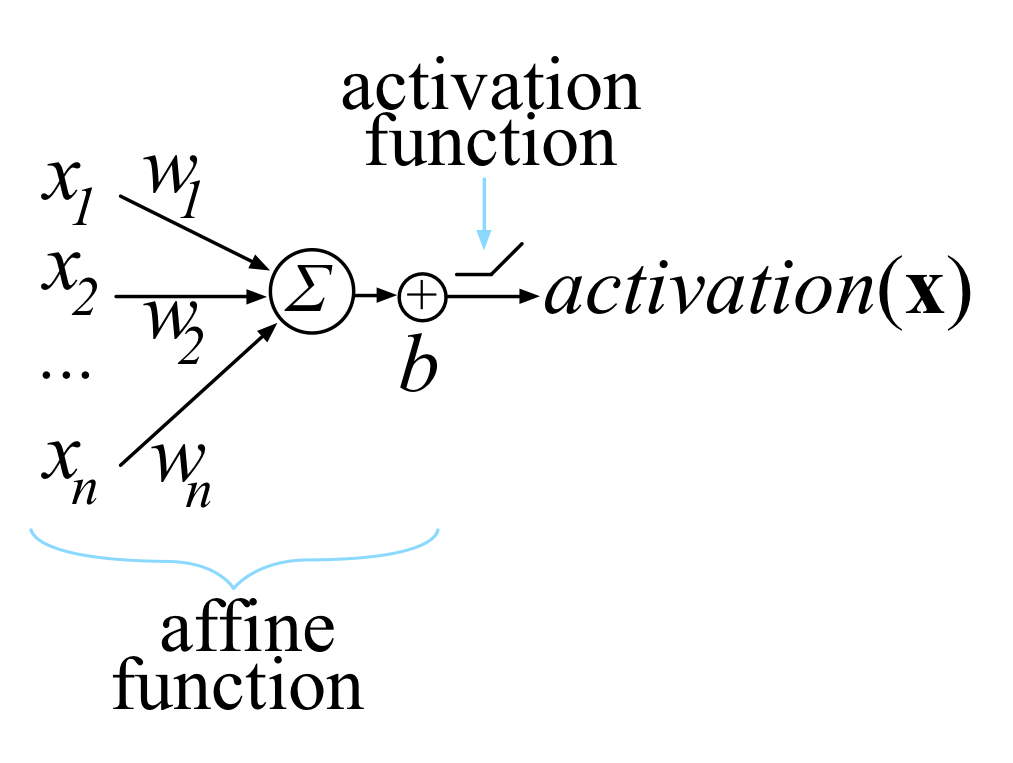
\includegraphics{neuron.png}
\end{center}

神经网络由许多这样的单元组成,这些单元被组织成称为{\em 层}的多个神经元集合。一层单元的激活值成为下一层单元的输入。最终层中单元或单元的激活值称为网络输出。

{\em 训练}这个神经元意味着选择权重 $\mathbf{w}$ 和偏置 $b$,使得对于所有 $N$ 个输入 $\mathbf{x}$,我们都能得到期望的输出。为了做到这一点,我们最小化一个{\em 损失函数},它将网络的最终 $activation(\mathbf{x})$ 与 $target(\mathbf{x})$(输入 $\mathbf{x}$ 的期望输出)进行比较,适用于所有输入向量 $\mathbf{x}$。为了最小化损失,我们使用梯度下降的一些变体,如普通的\href{https://en.wikipedia.org/wiki/Stochastic_gradient_descent}{随机梯度下降} (SGD)、带有动量的 SGD,或\href{https://en.wikipedia.org/wiki/Stochastic_gradient_descent\#Adam}{Adam}。所有这些方法都需要 $activation(\mathbf{x})$ 关于模型参数 $\mathbf{w}$ 和 $b$ 的偏导数(梯度)。我们的目标是逐渐调整 $\mathbf{w}$ 和 $b$,使得整体损失函数在所有 $\mathbf{x}$ 输入上不断减小。

如果我们谨慎一点,我们可以通过对一个常见的损失函数(均方误差)的标量版本进行求导来推导梯度:

\[
\frac{1}{N} \sum_{\mathbf{x}} (target(\mathbf{x}) - activation(\mathbf{x}))^2 = \frac{1}{N} \sum_{\mathbf{x}} (target(\mathbf{x}) - \max(0, \sum_i^{|x|} w_i x_i + b))^2
\]

但这只是一个神经元,神经网络必须同时训练所有层中所有神经元的权重和偏置。由于有多个输入和(可能的)多个网络输出,我们确实需要关于标量函数对向量求导以及向量值函数对向量求导的一些通用规则。

本文将推导一些关于向量求偏导的重要规则,特别是那些在训练神经网络时非常有用的规则。这个领域被称为{\em 矩阵微积分},好消息是,我们只需要其中一小部分,这部分内容我们将在本文中介绍。虽然网上有很多关于多元微积分和线性代数的材料,但它们通常是作为两门独立的本科课程来教授的,因此大多数材料将它们分开处理。那些讨论矩阵微积分的页面往往只是列出了一些规则,且解释很少,或者只是故事的一部分。此外,由于它们使用了密集的符号,并且对基础概念的讨论很少,这些材料对于除了少数数学家之外的大多数人来说,都相当晦涩。

(请参阅文末的注释资源列表。)

相比之下,我们将重新推导和重新发现一些关键的矩阵微积分规则,以便解释它们。事实证明,矩阵微积分其实并不难!不需要学习几十个新规则,只需要掌握几个关键概念。我们希望这篇短文能帮助你快速入门矩阵微积分,特别是将其应用于训练神经网络。我们假设你已经熟悉神经网络架构和训练的基础知识。如果你不熟悉,可以前往 \href{http://course.fast.ai}{Jeremy 的课程},完成第一部分,然后等你完成后我们再回来这里。(请注意,与许多更学术化的 approach 不同,我们强烈建议首先学习如何在实践中训练和使用神经网络,然后再研究底层数学。在上下文到位的情况下,数学将容易理解得多;而且,要成为一个有效的实践者,并不需要完全理解所有这些微积分知识。)

{\em 符号说明}: Jeremy 的课程仅使用代码,而不是数学符号,来解释概念,因为代码中不熟悉的函数很容易搜索和实验。在这篇论文中,我们相反:使用了大量的数学符号,因为本文的一个目标是帮助你理解在深度学习论文和书籍中看到的符号。在论文的 \href{\#notation}{末尾}, 你会发现一个简短的符号表,其中包括你可以用来搜索更多详细信息的单词或短语。


\section{回顾:标量导数规则}\label{sec2}

希望你还能记得一些主要的标量导数规则。如果你对这些规则有些模糊,可以看看 \href{https://www.khanacademy.org/math/ap-calculus-ab/ab-derivative-rules}{Khan Academy 关于标量导数规则的视频}。

\begin{tabular}{p{0.20\linewidth}lp{0.30\linewidth}l}
{\bf 规则}&{\bf $f(x)$}&{\bf 关于 $x$ 的标量导数表示法}&{\bf 例子}\\
{\bf 常数}&$c$&$0$&$\frac{d}{dx}99 = 0$\\
{\bf 常数乘法}&$cf$&$c \frac{df}{dx}$&$\frac{d}{dx}3x = 3$\\
{\bf 幂法则}&$x^n$&$nx^{n-1}$&$\frac{d}{dx}x^3 = 3x^2$\\
{\bf 求和法则}&$f + g$&$\frac{df}{dx} + \frac{dg}{dx}$&$\frac{d}{dx} (x^2 + 3x) = 2x + 3$\\
{\bf 差法则}&$f - g$&$\frac{df}{dx} - \frac{dg}{dx}$&$\frac{d}{dx}(x^2 - 3x) = 2x - 3$\\
{\bf 乘积法则}&$fg$&$f \frac{dg}{dx} + \frac{df}{dx} g$&$\frac{d}{dx}x^2x = x^2 + x2x = 3x^2$\\
{\bf 链式法则}&$f(g(x))$&$\frac{df(u)}{du}\frac{du}{dx}$, 令 $u=g(x)$&$\frac{d}{dx} \ln(x^2) = \frac{1}{x^2}2x = \frac{2}{x}$\\
\end{tabular}

还有其他关于三角函数、指数函数等的规则,你可以在 \href{https://www.khanacademy.org/math/differential-calculus}{Khan Academy 的微积分课程} 中找到。

当函数有一个参数,$f(x)$ 时,你常常会看到 $f'$ 和 $f'(x)$ 作为 $\frac{d}{dx}f(x)$ 的简写。我们建议不要使用这种记法,因为它没有明确指出是对哪个变量求导。

你可以将 $\frac{d}{dx}$ 看作是一个将一个参数的函数映射到另一个函数的操作符。也就是说,$\frac{d}{dx} f(x)$ 将 $f(x)$ 映射到它关于 $x$ 的导数,这与 $\frac{df(x)}{dx}$ 是同一个意思。另外,如果 $y = f(x)$,那么 $\frac{dy}{dx} = \frac{df(x)}{dx} = \frac{d}{dx}f(x)$。将导数视为操作符有助于简化复杂的导数计算,因为操作符是可分配的,并且允许我们将常数提出来。例如,在以下等式中,我们可以将常数 9 提出来,并将导数操作符分配到括号内的每一项。
\[
\frac{d}{dx} 9(x + x^2) = 9 \frac{d}{dx}(x + x^2) = 9 (\frac{d}{dx}x + \frac{d}{dx}x^2) = 9(1 + 2x) = 9 + 18x
\]
这个过程将 $9(x + x^2)$ 的导数简化为一些算术运算和 $x$ 与 $x^2$ 的导数,比原导数更容易求解。


\section{向量微积分和偏导数简介}\label{sec3}

神经网络层并不是单一参数的单函数 $f(x)$。因此,我们继续考虑多参数函数,如 $f(x, y)$。例如,$xy$(即 $x$ 和 $y$ 的乘积)的导数是什么?换句话说,当变量变化时,乘积 $xy$ 如何变化?这取决于我们是改变 $x$ 还是 $y$。我们一次对一个变量(参数)求导,为我们提供了两个不同的{\em 偏导数}(一个关于 $x$,一个关于 $y$)。

与使用算子 $\frac{d}{dx}$ 不同,偏导数算子是 $\frac{\partial}{\partial x}$(这是一个花体的 $d$,而不是希腊字母 $\delta$)。因此,$\frac{\partial }{\partial x}xy$ 和 $\frac{\partial }{\partial y}xy$ 是 $xy$ 的偏导数,通常简称为{\em 偏导数}。对于单参数函数,算子 $\frac{\partial}{\partial x}$ 等同于 $\frac{d}{dx}$(对于足够光滑的函数)。然而,最好使用 $\frac{d}{dx}$ 来明确表示标量导数。

关于 $x$ 的偏导数就是通常的标量导数,只是将方程中的其他变量视为常数。考虑函数 $f(x, y) = 3x^2y$。关于 $x$ 的偏导数写作 $\frac{\partial}{\partial x} 3x^2y$。从 $\frac{\partial}{\partial x}$ 的角度来看,3、2 和 $y$ 都是常数。因此,$\frac{\partial}{\partial x} 3yx^2 = 3y \frac{\partial}{\partial x} x^2 = 3y \cdot 2x = 6yx$。关于 $y$ 的偏导数将 $x$ 视为常数:$\frac{\partial}{\partial y} 3x^2y = 3x^2 \frac{\partial}{\partial y} y = 3x^2 \cdot 1 = 3x^2$。在继续之前,最好自己推导一下这些公式,否则接下来的内容可能难以理解。这里有一个关于偏导数的\href{https://www.khanacademy.org/math/multivariable-calculus/multivariable-derivatives/partial-derivative-and-gradient-articles/a/introduction-to-partial-derivatives}{Khan Academy 视频},如果需要帮助的话。

为了明确我们正在做向量微积分而不是多变量微积分,让我们考虑一下我们对 $f(x, y)$ 的偏导数 $\frac{\partial f(x, y)}{\partial x}$ 和 $\frac{\partial f(x, y)}{\partial y}$(另一种说法是 $\frac{\partial}{\partial x}f(x, y)$ 和 $\frac{\partial }{\partial y}f(x, y)$)所做的工作。而不是让它们无序地存在,我们把它们组织成一个水平向量。我们称这个向量为 $f(x, y)$ 的{\em 梯度},写作:
\[
\nabla f(x, y) = \left[ \frac{\partial f(x, y)}{\partial x}, \frac{\partial f(x, y)}{\partial y} \right] = [6yx, 3x^2]
\]
所以,$f(x, y)$ 的梯度仅仅是其偏导数的向量。梯度是向量微积分的一部分,它处理的是将 $n$ 个标量参数映射到单个标量的函数。现在,让我们考虑同时求多个函数的导数,这会很有趣。


\section{矩阵微积分}\label{sec4}

当我们从单个函数的导数过渡到多个函数的导数时,我们就从向量微积分的世界进入了矩阵微积分的世界。让我们为两个函数计算偏导数,这两个函数都接受两个参数。我们可以继续使用上一节中的 $f(x, y) = 3x^2y$,同时也引入 $g(x, y) = 2x + y^8$。$g$ 的梯度有两个分量,分别是每个参数的偏导数:

\[
\frac{\partial g(x,y)}{\partial x} = \frac{\partial 2x}{\partial x} + \frac{\partial y^8}{\partial x} = 2\frac{\partial x}{\partial x} + 0 = 2 \times 1 = 2
\]

和

\[
\frac{\partial g(x,y)}{\partial y} = \frac{\partial 2x}{\partial y} + \frac{\partial y^8}{\partial y} = 0 + 8y^7 = 8y^7
\]

因此,梯度为 $\nabla g(x,y) = [2, 8y^7]$。

梯度向量组织了特定标量函数的所有偏导数。如果我们有两个函数,我们可以通过堆叠它们的梯度来将它们的梯度组织成一个矩阵。当我们这样做时,我们得到{\em 雅可比矩阵}(或简称{\em 雅可比}),其中梯度是行向量:

\[
J =
\begin{bmatrix}
	\nabla f(x,y)\\
	\nabla g(x,y)
\end{bmatrix} = \begin{bmatrix}
 \frac{\partial f(x,y)}{\partial x} & \frac{\partial f(x,y)}{\partial y}\\
 \frac{\partial g(x,y)}{\partial x} & \frac{\partial g(x,y)}{\partial y}\\
\end{bmatrix} = \begin{bmatrix}
	6yx & 3x^2\\
	2 & 8y^7
\end{bmatrix}
\]

欢迎来到矩阵微积分的世界!

{\bf 注意,表示雅可比矩阵有多种方式。}我们使用所谓的\href{https://en.wikipedia.org/wiki/Matrix_calculus\#Layout_conventions}{分子布局},但许多论文和软件会使用{\em 分母布局}。分母布局的雅可比矩阵是分子布局雅可比矩阵的转置(沿对角线翻转):

\[
\begin{bmatrix}
	6yx & 2\\
	3x^2 & 8y^7
\end{bmatrix}
\]

\subsection{雅可比矩阵的推广}\label{sec4.1}

到目前为止,我们已经研究了一个具体的雅可比矩阵的例子。为了更一般地定义雅可比矩阵,我们将多个参数组合成一个单一的向量参数:$f(x, y, z) \Rightarrow f(\mathbf{x})$。(在文献中,有时会用符号$\vec{x}$表示向量。)用粗体小写字母表示向量,如$\mathbf{x}$,而用斜体小写字母表示标量,如$x$。$x_i$是向量$\mathbf{x}$的第$i$个元素,是标量,因此用斜体表示。我们还需要定义向量$\mathbf{x}$的方向。默认情况下,假设所有向量都是垂直的,大小为$n \times 1$:

\[
\mathbf{x} = \begin{bmatrix}
           x_1\\
           x_2\\
           \vdots \\
           x_n\\
           \end{bmatrix}
\]

对于多个标量函数,我们可以像处理参数一样将它们组合成一个向量。设$\mathbf{y} = \mathbf{f}(\mathbf{x})$是一个包含$m$个标量函数的向量,每个函数都接受一个长度为$n=|\mathbf{x}|$的向量$\mathbf{x}$作为输入,其中$|\mathbf{x}|$是向量$\mathbf{x}$中元素的个数。在$\mathbf{f}$中的每个函数$f_i$都返回一个标量,就像上一节中所做的那样:

\[
\begin{array}{lcl}
 y_1 & = & f_1(\mathbf{x})\\
 y_2 & = & f_2(\mathbf{x})\\
 & \vdots & \\
 y_m & = & f_m(\mathbf{x})\\
\end{array}
\]

例如,我们可以将上一节中的$f(x, y) = 3x^2y$和$g(x, y) = 2x + y^8$表示为:

\[
\begin{array}{lllllllll}
 y_1 = f_1(\mathbf{x}) = 3x_1^2x_2  &&&(\text{用$x_1$代替$x$,$x_2$代替$y$})\\
 y_2 = f_2(\mathbf{x}) = 2x_1 + x_2^8
\end{array}
\]

通常情况下,$m = n$,因为我们对于$\mathbf{x}$向量的每个元素都有一个标量函数结果。例如,考虑恒等函数$\mathbf{y} = \mathbf{f(x)} = \mathbf{x}$:

\[
\begin{array}{lclcc}
 y_1 & = & f_1(\mathbf{x})& = & x_1\\
 y_2 & = & f_2(\mathbf{x})& = & x_2\\
 & \vdots & \\
 y_n & = & f_n(\mathbf{x})& = & x_n\\
\end{array}
\]

在这种情况下,我们有$m = n$个函数和参数。一般来说,雅可比矩阵包含所有可能的$m \times n$个偏导数($m$行,$n$列),即$m$个关于$\mathbf{x}$的梯度的堆栈:

\[
\frac{\partial \mathbf{y}}{\partial \mathbf{x}} = \begin{bmatrix}
\nabla f_1(\mathbf{x}) \\
\nabla f_2(\mathbf{x})\\
\ldots\\
\nabla f_m(\mathbf{x})
\end{bmatrix} = \begin{bmatrix}
\frac{\partial}{\partial \mathbf{x}} f_1(\mathbf{x}) \\
\frac{\partial}{\partial \mathbf{x}} f_2(\mathbf{x})\\
\ldots\\
\frac{\partial}{\partial \mathbf{x}} f_m(\mathbf{x})
\end{bmatrix} = \begin{bmatrix}
\frac{\partial}{\partial {x_1}} f_1(\mathbf{x})~ \frac{\partial}{\partial {x_2}} f_1(\mathbf{x}) ~\ldots~ \frac{\partial}{\partial {x_n}} f_1(\mathbf{x}) \\
\frac{\partial}{\partial {x_1}} f_2(\mathbf{x})~ \frac{\partial}{\partial {x_2}} f_2(\mathbf{x}) ~\ldots~ \frac{\partial}{\partial {x_n}} f_2(\mathbf{x}) \\
\ldots\\
~\frac{\partial}{\partial {x_1}} f_m(\mathbf{x})~ \frac{\partial}{\partial {x_2}} f_m(\mathbf{x}) ~\ldots~ \frac{\partial}{\partial {x_n}} f_m(\mathbf{x}) \\
\end{bmatrix}
\]

每个$\frac{\partial}{\partial \mathbf{x}} f_i(\mathbf{x})$是一个横向的$n$维向量,因为偏导数是对长度为$n = |\mathbf{x}|$的向量$\mathbf{x}$求导。因此,雅可比矩阵的宽度是$n$,因为我们对$\mathbf{x}$求偏导数,有$n$个参数可以改变,每个参数可能改变函数的值。因此,雅可比矩阵总是有$m$行,对应$m$个方程。通过可视化可能的雅可比矩阵形状,有助于理解:

\begin{center}

\begin{tabular}{c|ccl}
  & \begin{tabular}[t]{c}
  标量\\
  \framebox(18,18){$x$}\\
  \end{tabular} & \begin{tabular}{c}
  向量\\
  \framebox(18,40){$\mathbf{x}$}
  \end{tabular}\\
\hline
\\[\dimexpr-\normalbaselineskip+5pt]
\begin{tabular}[b]{c}
  标量\\
  \framebox(18,18){$f$}\\
  \end{tabular} &\framebox(18,18){$\frac{\partial f}{\partial {x}}$} & \framebox(40,18){$\frac{\partial f}{\partial {\mathbf{x}}}$}&\\
\begin{tabular}[b]{c}
  向量\\
  \framebox(18,40){$\mathbf{f}$}\\
  \end{tabular} & \framebox(18,40){$\frac{\partial \mathbf{f}}{\partial {x}}$} & \framebox(40,40){$\frac{\partial \mathbf{f}}{\partial \mathbf{x}}$}\\
\end{tabular}

\end{center}

恒等函数$\mathbf{f(x)} = \mathbf{x}$的雅可比矩阵,其中$f_i(\mathbf{x}) = x_i$,有$n$个函数,每个函数有$n$个参数,存储在一个向量$\mathbf{x}$中。因此,雅可比矩阵是一个方阵,因为$m = n$:

\begin{center}

\begin{eqnarray*}
	\frac{\partial \mathbf{y}}{\partial \mathbf{x}} = \begin{bmatrix}
	\frac{\partial}{\partial \mathbf{x}} f_1(\mathbf{x}) \\
	\frac{\partial}{\partial \mathbf{x}} f_2(\mathbf{x})\\
	\ldots\\
	\frac{\partial}{\partial \mathbf{x}} f_m(\mathbf{x})
	\end{bmatrix} &=& \begin{bmatrix}
	\frac{\partial}{\partial {x_1}} f_1(\mathbf{x})~ \frac{\partial}{\partial {x_2}} f_1(\mathbf{x}) ~\ldots~  \frac{\partial}{\partial {x_n}} f_1(\mathbf{x}) \\
	\frac{\partial}{\partial {x_1}} f_2(\mathbf{x})~ \frac{\partial}{\partial {x_2}} f_2(\mathbf{x}) ~\ldots~  \frac{\partial}{\partial {x_n}} f_2(\mathbf{x}) \\
	\ldots\\
	~\frac{\partial}{\partial {x_1}} f_m(\mathbf{x})~ \frac{\partial}{\partial {x_2}} f_m(\mathbf{x}) ~\ldots~ \frac{\partial}{\partial {x_n}} f_m(\mathbf{x}) \\
	\end{bmatrix}\\\\
	& = & \begin{bmatrix}
	\frac{\partial}{\partial {x_1}} x_1~ \frac{\partial}{\partial {x_2}} x_1 ~\ldots~ \frac{\partial}{\partial {x_n}} x_1 \\
	\frac{\partial}{\partial {x_1}} x_2~ \frac{\partial}{\partial {x_2}} x_2 ~\ldots~ \frac{\partial}{\partial {x_n}} x_2 \\
	\ldots\\
	~\frac{\partial}{\partial {x_1}} x_n~ \frac{\partial}{\partial {x_2}} x_n ~\ldots~ \frac{\partial}{\partial {x_n}} x_n \\
	\end{bmatrix}\\\\
	& & (\text{并且由于 } \frac{\partial}{\partial {x_j}} x_i = 0 \text{ 当 } j \neq i)\\
	 & = & \begin{bmatrix}
	\frac{\partial}{\partial {x_1}} x_1 & 0 & \ldots& 0 \\
	0 & \frac{\partial}{\partial {x_2}} x_2 &\ldots & 0 \\
	& & \ddots\\
	0 & 0 &\ldots& \frac{\partial}{\partial {x_n}} x_n \\
	\end{bmatrix}\\\\
	 & = & \begin{bmatrix}
	1 & 0 & \ldots& 0 \\
	0 &1 &\ldots & 0 \\
	& & \ddots\\
	0 & 0 & \ldots &1 \\
	\end{bmatrix}\\\\
	& = & I ~~~(I \text{ 是对角线为1的单位矩阵})\\
	\end{eqnarray*}

\end{center}

在继续之前,确保你能推导出上述每一步。如果遇到困难,只需单独考虑矩阵的每个元素,并应用常规的标量导数规则。这是一个普遍有用的技巧:将向量表达式分解为一组标量表达式,然后对所有偏导数进行求导,在最后适当地将结果组合成向量和矩阵。

还要小心区分矩阵是垂直的$\mathbf{x}$还是水平的$\mathbf{x}^T$,其中$\mathbf{x}^T$表示$\mathbf{x}$的转置。同时,注意区分标量函数$y = ...$和向量函数(或向量值函数)$\mathbf{y} = ...$。

\subsection{向量逐元素二元运算的导数}\label{sec4.2}

向量上的逐元素二元运算,如向量加法 $\mathbf{w} + \mathbf{x}$,非常重要,因为我们可以用这些运算来表示许多常见的向量操作,例如向量与标量的乘法。所谓“逐元素二元运算”就是指对每个向量的第一个元素应用运算符得到输出的第一个元素,对第二个元素应用运算符得到输出的第二个元素,依此类推。例如,在numpy或tensorflow中,默认情况下所有基本数学运算都是以这种方式应用的。在深度学习中常见的例子有 $max(\mathbf{w},\mathbf{x})$ 和 $\mathbf{w} > \mathbf{x}$(返回一个由1和0组成的向量)。

我们可以用符号 $\mathbf{y} = \mathbf{f(w)} \bigcirc \mathbf{g(x)}$ 来表示逐元素二元运算,其中 $m=n=|y|=|w|=|x|$。(注意:$|x|$表示$x$中的元素个数。)符号$\bigcirc$表示任何逐元素运算符(如$+$),而不是函数复合运算符$\circ$。下面是当我们放大查看标量方程时,方程 $\mathbf{y} = \mathbf{f(w)} \bigcirc \mathbf{g(x)}$ 的样子:

\[
\begin{bmatrix}
           y_1\\
           y_2\\
           \vdots \\
           y_n\\
           \end{bmatrix} = \begin{bmatrix}
           f_{1}(\mathbf{w}) \bigcirc g_{1}(\mathbf{x})\\
           f_{2}(\mathbf{w}) \bigcirc g_{2}(\mathbf{x})\\
           \vdots \\
           f_{n}(\mathbf{w}) \bigcirc g_{n}(\mathbf{x})\\
         \end{bmatrix}
\]

其中我们垂直写出了$n$(而不是$m$)个方程,以强调逐元素运算的结果是一个大小为$m=n$的向量。

根据上一节的思想,我们可以看到关于$\mathbf{w}$的雅可比矩阵的一般情况是:

\[
J_\mathbf{w} = 
\frac{\partial \mathbf{y}}{\partial \mathbf{w}}  = \begin{bmatrix}
\frac{\partial}{\partial w_1} ( f_{1}(\mathbf{w}) \bigcirc g_{1}(\mathbf{x}) ) & \frac{\partial}{\partial w_2} ( f_{1}(\mathbf{w}) \bigcirc g_{1}(\mathbf{x}) ) & \ldots & \frac{\partial}{\partial w_n} ( f_{1}(\mathbf{w}) \bigcirc g_{1}(\mathbf{x}) )\\
\frac{\partial}{\partial w_1} ( f_{2}(\mathbf{w}) \bigcirc g_{2}(\mathbf{x}) ) & \frac{\partial}{\partial w_2} ( f_{2}(\mathbf{w}) \bigcirc g_{2}(\mathbf{x}) ) & \ldots & \frac{\partial}{\partial w_n} ( f_{2}(\mathbf{w}) \bigcirc g_{2}(\mathbf{x}) )\\
& \ldots\\
\frac{\partial}{\partial w_1} ( f_{n}(\mathbf{w}) \bigcirc g_{n}(\mathbf{x}) ) & \frac{\partial}{\partial w_2} ( f_{n}(\mathbf{w}) \bigcirc g_{n}(\mathbf{x}) ) & \ldots & \frac{\partial}{\partial w_n} ( f_{n}(\mathbf{w}) \bigcirc g_{n}(\mathbf{x}) )\\
\end{bmatrix}
\]

而关于$\mathbf{x}$的雅可比矩阵是:

\[
J_\mathbf{x} = 
\frac{\partial \mathbf{y}}{\partial \mathbf{x}}  = \begin{bmatrix}
\frac{\partial}{\partial x_1} ( f_{1}(\mathbf{w}) \bigcirc g_{1}(\mathbf{x}) ) & \frac{\partial}{\partial x_2} ( f_{1}(\mathbf{w}) \bigcirc g_{1}(\mathbf{x}) ) & \ldots & \frac{\partial}{\partial x_n} ( f_{1}(\mathbf{w}) \bigcirc g_{1}(\mathbf{x}) )\\
\frac{\partial}{\partial x_1} ( f_{2}(\mathbf{w}) \bigcirc g_{2}(\mathbf{x}) ) & \frac{\partial}{\partial x_2} ( f_{2}(\mathbf{w}) \bigcirc g_{2}(\mathbf{x}) ) & \ldots & \frac{\partial}{\partial x_n} ( f_{2}(\mathbf{w}) \bigcirc g_{2}(\mathbf{x}) )\\
& \ldots\\
\frac{\partial}{\partial x_1} ( f_{n}(\mathbf{w}) \bigcirc g_{n}(\mathbf{x}) ) & \frac{\partial}{\partial x_2} ( f_{n}(\mathbf{w}) \bigcirc g_{n}(\mathbf{x}) ) & \ldots & \frac{\partial}{\partial x_n} ( f_{n}(\mathbf{w}) \bigcirc g_{n}(\mathbf{x}) )\\
\end{bmatrix}
\]

这确实很复杂,但幸运的是,雅可比矩阵通常是一个对角矩阵,即除了对角线元素外,其余元素都为零。因为这极大地简化了雅可比矩阵,所以我们需要详细研究在逐元素运算中,雅可比矩阵何时简化为对角矩阵。

在对角雅可比矩阵中,所有非对角线元素都为零,即 $\frac{\partial}{\partial w_j} ( f_i(\mathbf{w}) \bigcirc g_i(\mathbf{x}) ) = 0$,其中 $j \neq i$。(注意,我们是对 $w_j$ 求偏导,而不是 $w_i$。)在什么条件下这些非对角线元素为零?当 $f_i$ 和 $g_i$ 对 $w_j$ 来说是常数时,即 $\frac{\partial}{\partial w_j} f_i(\mathbf{w}) = \frac{\partial}{\partial w_j} g_i(\mathbf{x}) = 0$。

无论运算符是什么,如果这些偏导数为零,那么运算结果也为零,$0 \bigcirc 0 = 0$,并且常数的偏导数为零。

当 $f_i$ 和 $g_i$ 不是 $w_j$ 的函数时,这些偏导数为零。我们知道,逐元素运算意味着 $f_i$ 只是 $w_i$ 的函数,$g_i$ 只是 $x_i$ 的函数。例如,$\mathbf{w} + \mathbf{x}$ 的逐元素求和是 $w_i + x_i$。因此,$f_i(\mathbf{w}) \bigcirc g_i(\mathbf{x})$ 可以简化为 $f_i(w_i) \bigcirc g_i(x_i)$,目标是求 $\frac{\partial}{\partial w_j} f_i(w_i) = \frac{\partial}{\partial w_j} g_i(x_i) = 0$。对于 $j \neq i$,$f_i(w_i)$ 和 $g_i(x_i)$ 对 $\partial w_j$ 来说是常数,因此非对角线上的偏导数为零。

(注意:$f_i(w_i)$ 在技术上是滥用符号,因为$f_i$和$g_i$是向量函数,而不是单个元素的函数。不过为了简化,我们继续使用这个记法。)

在这种条件下,雅可比矩阵的对角线元素是 $\frac{\partial}{\partial w_i} ( f_i(w_i) \bigcirc g_i(x_i) )$:

\[
\frac{\partial \mathbf{y}}{\partial \mathbf{w}}  = \begin{bmatrix}
\frac{\partial}{\partial w_1} ( f_{1}(w_1) \bigcirc g_{1}(x_1) )\\
& \frac{\partial}{\partial w_2} (f_{2}(w_2) \bigcirc g_{2}(x_2) ) & & \text{\huge0}\\
& & \ldots \\
\text{\huge0}& & & \frac{\partial}{\partial w_n} (f_{n}(w_n) \bigcirc g_{n}(x_n) )
\end{bmatrix}
\]

(大写的“0”表示所有非对角线元素为0。)

更简洁地,我们可以写成:

\[
\frac{\partial \mathbf{y}}{\partial \mathbf{w}} = diag \left( \frac{\partial}{\partial w_1}(f_{1}(w_1) \bigcirc g_{1}(x_1)),~ \frac{\partial}{\partial w_2}(f_{2}(w_2) \bigcirc g_{2}(x_2)),~ \ldots,~ \frac{\partial}{\partial w_n}(f_{n}(w_n) \bigcirc g_{n}(x_n)) \right)
\]

和

\[
\frac{\partial \mathbf{y}}{\partial \mathbf{x}} = diag \left( \frac{\partial}{\partial x_1}(f_{1}(w_1) \bigcirc g_{1}(x_1)),~ \frac{\partial}{\partial x_2}(f_{2}(w_2) \bigcirc g_{2}(x_2)),~ \ldots,~ \frac{\partial}{\partial x_n}(f_{n}(w_n) \bigcirc g_{n}(x_n)) \right)
\]

其中 $diag(\mathbf{x})$ 表示一个对角矩阵,其对角线元素取自向量 $\mathbf{x}$。

由于我们经常进行简单的向量算术运算,因此在二元逐元素运算中,一般的函数 $\mathbf{f(w)}$ 往往就是向量 $\mathbf{w}$ 本身。每当一般的函数是一个向量时,我们知道 $f_i(\mathbf{w})$ 可以简化为 $f_i(w_i) = w_i$。例如,向量加法 $\mathbf{w + x}$ 满足逐元素对角条件,因为 $\mathbf{f(w)} + \mathbf{g(x)}$ 的标量方程 $y_i = f_i(\mathbf{w}) + g_i(\mathbf{x})$ 可以简化为 $y_i = f_i(w_i) + g_i(x_i) = w_i + x_i$,其偏导数为:

\[
\frac{\partial}{\partial w_i} ( f_{i}(w_i) + g_{i}(x_i) ) = \frac{\partial}{\partial w_i}(w_i + x_i) = 1 + 0 = 1
\]

\[
\frac{\partial}{\partial x_i} ( f_{i}(w_i) + g_{i}(x_i) ) = \frac{\partial}{\partial x_i}(w_i + x_i) = 0 + 1 = 1
\]

因此,$\frac{\partial (\mathbf{w+x})}{\partial \mathbf{w}} = \frac{\partial (\mathbf{w+x})}{\partial \mathbf{x}} = I$,即单位矩阵,因为对角线上的每个元素都是1。$I$ 表示适当维度的单位矩阵,除了对角线上的1,其余元素均为0。

鉴于这种特殊情况的简单性,$f_i(\mathbf{w})$ 简化为 $f_i(w_i)$,你应该能够推导出向量逐元素二元运算的常见雅可比矩阵:

\[
\begin{array}{lllllllll}
        \text{\bf{运算}} &  & {\text{\bf 关于 }} \mathbf{w} \text{ 的偏导数} \\
        + &  & \frac{\partial (\mathbf{w+x})}{\partial \mathbf{w}} = diag(\ldots \frac{\partial (w_i + x_i)}{\partial w_i} \ldots) = diag(\vec{1}) = I \\\\
        - &  & \frac{\partial (\mathbf{w-x})}{\partial \mathbf{w}}  =  diag(\ldots\frac{\partial (w_i - x_i)}{\partial w_i}\ldots) =  diag(\vec{1})  =  I \\\\
        \otimes &  & \frac{\partial (\mathbf{w \otimes x})}{\partial \mathbf{w}}  =  diag(\ldots\frac{\partial (w_i \times x_i)}{\partial w_i} \ldots)  =  diag(\mathbf{x}) \\\\
        \oslash &  & \frac{\partial (\mathbf{w \oslash x})}{\partial \mathbf{w}}  =  diag(\ldots\frac{\partial (w_i / x_i)}{\partial w_i}\ldots)  =  diag(\ldots \frac{1}{x_i} \ldots) \\\\
\end{array}
\]

\[
\begin{array}{lllllllll}
        \text{\bf{运算}} &  &  {\text{\bf 关于 }}\mathbf{x} \text{ 的偏导数}\\
        + &  & \frac{\partial (\mathbf{w+x})}{\partial \mathbf{x}} =  I\\\\
        - &  & \frac{\partial (\mathbf{w-x})}{\partial \mathbf{x}}  =  diag(\ldots\frac{\partial (w_i - x_i)}{\partial x_i}\ldots)  =  diag(-\vec{1})  =  -I \\\\
        \otimes &  &  \frac{\partial (\mathbf{w \otimes x})}{\partial \mathbf{x}}  =  diag(\mathbf{w})\\\\
        \oslash &  &  \frac{\partial (\mathbf{w \oslash x})}{\partial \mathbf{x}}  =  diag(\ldots \frac{-w_i}{x_i^2} \ldots)\\
\end{array}
\]

运算符$\otimes$和$\oslash$分别表示逐元素乘法和除法;$\otimes$有时称为{\em 哈达玛积}。逐元素乘法和除法没有标准的符号表示,因此我们采用与一般二元运算符表示法一致的方法。


\subsection{涉及标量扩展的导数}\label{sec4.3}

当我们对向量进行标量乘法或加法时,我们隐式地将标量扩展为向量,然后进行逐元素的二元运算。例如,将标量 $z$ 加到向量 $\mathbf{x}$ 上,即 $\mathbf{y} = \mathbf{x} + z$,实际上是 $\mathbf{y} = \mathbf{f(x)} + \mathbf{g}(z)$,其中 $\mathbf{f(x)} = \mathbf{x}$ 和 $\mathbf{g}(z) = \vec{1} z$。(符号 $\vec{1}$ 表示适当长度的全1向量。)$z$ 是不依赖于 $\mathbf{x}$ 的任意标量,这很有用,因为对于任何 $x_i$,都有 $\frac{\partial z}{\partial x_i} = 0$,从而简化我们的偏导数计算。(在这里,可以把变量 $z$ 看作常数。)类似地,标量乘法 $\mathbf{y} = \mathbf{x} z$ 实际上是 $\mathbf{y} = \mathbf{f(x)} \otimes \mathbf{g}(z) = \mathbf{x} \otimes \vec{1}z$,其中 $\otimes$ 是两个向量的逐元素乘法(Hadamard积)。

向量标量加法和乘法关于向量 $\mathbf{x}$ 的偏导数使用我们的逐元素规则:
\[ \frac{\partial \mathbf{y}}{\partial \mathbf{x}} = diag \left( \ldots \frac{\partial}{\partial x_i} ( f_i(x_i) \bigcirc g_i(z) ) \ldots \right) \]
这是因为函数 $\mathbf{f(x)} = \mathbf{x}$ 和 $\mathbf{g}(z) = \vec{1} z$ 明显满足雅可比矩阵的逐元素对角线条件(即 $f_i(\mathbf{x})$ 最多依赖于 $x_i$,而 $g_i(z)$ 依赖于 $\vec{1}z$ 向量的第 $i$ 个值)。

根据标量偏导数的常规规则,我们得到了向量标量加法的雅可比矩阵的对角线元素:
\[ \frac{\partial}{\partial x_i} ( f_i(x_i) + g_i(z) ) = \frac{\partial (x_i + z)}{\partial x_i} = \frac{\partial x_i}{\partial x_i} + \frac{\partial z}{\partial x_i} = 1 + 0 = 1 \]
因此,$\frac{\partial}{\partial \mathbf{x}} ( \mathbf{x} + z ) = diag(\vec{1}) = I$。

然而,关于标量参数 $z$ 的偏导数是一个垂直向量,而不是对角矩阵。向量的元素为:
\[ \frac{\partial}{\partial z} ( f_i(x_i) + g_i(z) ) = \frac{\partial (x_i + z)}{\partial z} = \frac{\partial x_i}{\partial z} + \frac{\partial z}{\partial z} = 0 + 1 = 1 \]
因此,$\frac{\partial}{\partial z} ( \mathbf{x} + z ) = \vec{1}$。

向量标量乘法的雅可比矩阵的对角线元素涉及标量导数的乘积法则:
\[ \frac{\partial}{\partial x_i} ( f_i(x_i) \otimes g_i(z) ) = x_i  \frac{\partial z}{\partial x_i} + z  \frac{\partial x_i}{\partial x_i} = 0 + z = z \]
因此,$\frac{\partial}{\partial \mathbf{x}} ( \mathbf{x} z ) = diag(\vec{1}  z) = I z$。

关于标量参数 $z$ 的偏导数是一个垂直向量,其元素为:
\[ \frac{\partial}{\partial z} ( f_i(x_i) \otimes g_i(z) ) = x_i \frac{\partial z}{\partial z} + z \frac{\partial x_i}{\partial z} = x_i + 0 = x_i \]
这给出了 $\frac{\partial}{\partial z} ( \mathbf{x} z ) = \mathbf{x}$。


\subsection{向量求和缩减}\label{sec4.4}

向量元素的求和是深度学习中的一个重要操作,例如网络损失函数,但也可以将其作为一种简化计算向量点积导数和其他将向量缩减为标量的操作的方法。

设 $y = \sum( \mathbf{f}(\mathbf{x})) = \sum_{i=1}^n f_i(\mathbf{x})$。注意这里我们仔细地将参数保留为向量 $\mathbf{x}$,因为每个函数 $f_i$ 可能会使用向量中的所有值,而不仅仅是 $x_i$。求和是对函数的{\bf 结果}进行的,而不是对参数进行的。向量求和的梯度($1 \times n$ 雅可比矩阵)为:
\[
\begin{array}{lcllll}
 \frac{\partial y}{\partial \mathbf{x}} & = & \begin{bmatrix} \frac{\partial y}{\partial x_1}, \frac{\partial y}{\partial x_2}, \ldots, \frac{\partial y}{\partial x_n} \end{bmatrix}\\\\
  & = & \begin{bmatrix} \frac{\partial}{\partial x_1} \sum_i f_i(\mathbf{x}),~ \frac{\partial}{\partial x_2} \sum_i f_i(\mathbf{x}),~ \ldots,~ \frac{\partial}{\partial x_n} \sum_i  f_i(\mathbf{x}) \end{bmatrix} \\\\
 & = & \begin{bmatrix} \sum_i \frac{\partial f_i(\mathbf{x})}{\partial x_1},~ \sum_i \frac{\partial f_i(\mathbf{x})}{\partial x_2},~ \ldots,~ \sum_i \frac{\partial f_i(\mathbf{x})}{\partial x_n}  \end{bmatrix}&&&(\text{将导数移到求和号内})\\
\end{array}
\]
(梯度元素内的求和可能会有些棘手,所以请确保保持一致的符号表示。)

我们来看一个简单的例子,$y = \sum(\mathbf{x})$ 的梯度。求和内部的函数仅仅是 $f_i(\mathbf{x}) = x_i$,因此梯度为:
\[\nabla y = \begin{bmatrix} \sum_i \frac{\partial f_i(\mathbf{x})}{\partial x_1},~ \sum_i \frac{\partial f_i(\mathbf{x})}{\partial x_2},~ \ldots,~ \sum_i \frac{\partial f_i(\mathbf{x})}{\partial x_n}  \end{bmatrix} = \begin{bmatrix} \sum_i \frac{\partial x_i}{\partial x_1},~ \sum_i \frac{\partial x_i}{\partial x_2},~ \ldots,~ \sum_i \frac{\partial x_i}{\partial x_n}  \end{bmatrix}\]
由于 $\frac{\partial}{\partial x_j} x_i = 0$ 当 $j \neq i$,我们可以简化为:
\[\nabla y = \begin{bmatrix} \frac{\partial x_1}{\partial x_1},~ \frac{\partial x_2}{\partial x_2},~ \ldots,~ \frac{\partial x_n}{\partial x_n}  \end{bmatrix} = \begin{bmatrix}1, 1, \ldots, 1\end{bmatrix} = \vec{1}^T\]
注意,结果是一个全为1的横向向量,而不是纵向向量,因此梯度是 $\vec{1}^T$。($\vec{1}^T$ 中的 $T$ 表示向量的转置。在这种情况下,它将一个纵向向量转换为横向向量。)保持所有向量和矩阵的形状是非常重要的,否则就无法计算复杂函数的导数。

再举一个例子,假设我们对一个向量与一个常数标量的乘积求和。如果 $y = \sum(\mathbf{x} z)$,那么 $f_i(\mathbf{x},z) = x_i z$,梯度为:
\[\begin{array}{lcl}
 \frac{\partial y}{\partial \mathbf{x}} & = & \begin{bmatrix} \sum_i \frac{\partial}{\partial x_1} x_i z,~ \sum_i \frac{\partial }{\partial x_2} x_i z,~ \ldots,~ \sum_i \frac{\partial}{\partial x_n} x_i z  \end{bmatrix}\\\\
 & = & \begin{bmatrix} \frac{\partial}{\partial x_1} x_1 z,~ \frac{\partial }{\partial x_2} x_2 z,~ \ldots,~ \frac{\partial}{\partial x_n} x_n z  \end{bmatrix}\\\\
 & = & \begin{bmatrix} z, z, \ldots, z \end{bmatrix}\\
\end{array}\]
关于标量变量 $z$ 的导数是一个 $1 \times 1$ 的量:
\[\begin{array}{lcl}
 \frac{\partial y}{\partial z} & = & \frac{\partial}{\partial z} \sum_{i=1}^n x_i z\\\\
 & = & \sum_i \frac{\partial}{\partial z} x_i z\\\\
 & = & \sum_i x_i\\\\
 & = & \sum(\mathbf{x})\\
\end{array}\]

\subsection{链式法则}\label{sec4.5}

我们无法仅使用迄今所见的基本矩阵微积分规则来计算非常复杂函数的偏导数。例如,我们不能直接对像 $\text{sum}(\mathbf{w} + \mathbf{x})$ 这样的嵌套表达式求导,而不将其还原为其标量等价物。我们需要能够结合我们的基本向量规则,使用我们所说的 {\em 向量链式法则}。不幸的是,有许多微分规则都被称为“链式法则”,所以我们必须小心我们所谈论的是哪一种链式法则。我们的目标之一是清晰地定义和命名三种不同的链式法则,并指出它们在哪些情况下适用。为了热身,我们将从我们所说的 {\em 单变量链式法则} 开始,即我们要计算标量函数关于标量的导数。然后我们将介绍一个重要的概念,即 {\em 全导数},并用它来定义我们严谨地称为 {\em 单变量全导数链式法则} 的内容。最后,我们将为神经网络准备全面的向量链式法则。

链式法则在概念上是一种分而治之的策略(类似于快速排序),它将复杂的表达式分解为导数更容易计算的子表达式。它的威力来自于我们能够独立处理每个简单的子表达式,同时仍然能够结合中间结果来得到正确的整体结果。

当我们需要一个由嵌套子表达式组成的表达式的导数时,链式法则就派上用场了。例如,在面对像 $\frac{d}{dx} \sin(x^2)$ 这样的表达式时,我们需要链式法则。最外层的表达式是对一个中间结果取 $\sin$,而这个嵌套的子表达式是对 $x$ 平方。具体来说,我们需要单变量链式法则,所以让我们从更详细地探讨这个开始。


\subsubsection{单变量链式法则}\label{sec4.5.1}

我们从求解嵌套表达式的导数开始:$\frac{d}{dx} \sin(x^2) = 2x\cos(x^2)$。不难看出,解中包含了标量微分规则的成分,如$\frac{d}{dx}x^2 = 2x$和$\frac{d}{du} \sin(u) = \cos(u)$。看起来,解法是将外层表达式的导数乘以内层表达式的导数,或者“将各部分连接起来”,这正是正确的做法。在本节中,我们将探讨工作的基本原则,并提供一个适用于单变量高度嵌套表达式的流程。

链式法则通常用嵌套函数来定义,例如对于单变量链式法则,$y = f(g(x))$。 (您还会看到用函数复合$(f \circ g)(x)$定义链式法则,这是同一个概念。)有些资料使用简写符号$y' = f'(g(x))g'(x)$来表示导数,但这掩盖了我们引入中间变量的事实:$u = g(x)$,我们稍后会看到这一点。最好显式地定义单变量链式法则,这样我们永远不会对错误的变量求导。这是我们推荐的单变量链式法则的公式:

\[
\frac{dy}{dx} = \frac{dy}{du}\frac{du}{dx}
\]

要应用单变量链式法则,请按照以下步骤进行:

\begin{enumerate}
\item 引入嵌套子表达式和二元及一元运算符的中间变量;例如,$\times$是二元运算符,$sin(x)$和其它三角函数通常是 unary,因为它们只有一个操作数。这一步将所有方程标准化为单个运算符或函数应用。
\item 计算中间变量相对于其参数的导数。
\item 通过将所有中间变量的导数相乘来组合,以获得整体结果。
\item 如果导数方程中引用了中间变量,则将其替换回来。
\end{enumerate}

第三步将“链”放入“链式法则”,因为它将中间结果连接在一起。将中间导数相乘是链式法则所有变体的共同主题。

让我们尝试将这个过程应用于 $y = f(g(x)) = \sin(x^2)$:

\begin{enumerate}
\item 引入中间变量。设 $u = x^2$ 表示子表达式 $x^2$(简写为 $u(x) = x^2$)。这给出了:

\[
\begin{array}{lllll}
  u &=& x^2 &&(\text{相对于定义 }f(g(x)), g(x) = x^2)\\
  y &=& \sin(u) && (y = f(u) = \sin(u))
\end{array}
\]

这些子表达式的顺序不影响答案,但我们建议按照嵌套所规定的逆向操作顺序进行(从内到外)。这样,表达式和导数始终是之前计算元素的函数。
\item 计算导数。

\[
\begin{array}{lllll}
 \frac{du}{dx} &=& 2x && (\text{对 }x \text{ 求导})\\
 \frac{dy}{du} &=& \cos(u) && (\text{对 }u \text{ 求导,而不是 }x)
\end{array}
\]

\item 结合。

\[
\frac{dy}{dx} = \frac{dy}{du} \frac{du}{dx} = \cos(u)2x
\]

\item 替换。

\[
\frac{dy}{dx} = \frac{dy}{du} \frac{du}{dx} = \cos(x^2)2x = 2x\cos(x^2)
\]
\end{enumerate}

请注意,单独计算中间变量的导数是多么容易!链式法则说这样做是合法的,并告诉我们如何结合中间结果以得到 $2x\cos(x^2)$。

你可以将链式法则的结合步骤理解为单位消去。如果我们让 $y$ 表示英里,$x$ 表示油箱中的加仑数,$u$ 表示加仑,我们可以将 $\frac{dy}{dx} = \frac{dy}{du} \frac{du}{dx}$ 解释为 $\frac{miles}{tank} = \frac{miles}{gallon} \frac{gallon}{tank}$。加仑的分母和分子相互抵消。

另一种思考单变量链式法则的方式是将整体表达式可视化为数据流图或操作链(或编译器人员的抽象语法树):

\begin{center}
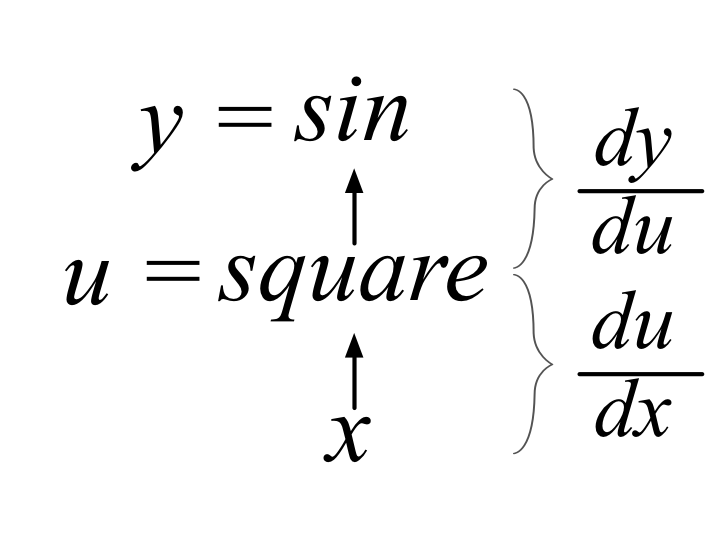
\includegraphics{sin-square.png}
\end{center}

函数参数 $x$ 的变化通过平方操作传递,然后再通过 $sin$ 操作传递,从而改变结果 $y$。你可以将 $\frac{du}{dx}$ 看作是从 $x$ 到 $u$ 的变化,将 $\frac{dy}{du}$ 看作是从 $u$ 到 $y$ 的变化。从 $x$ 到 $y$ 需要一个中间步骤。按照惯例,链式法则通常从输出变量写到参数,即 $\frac{dy}{dx} = \frac{dy}{du} \frac{du}{dx}$。但是,如果我们反过来,使用等效的 $\frac{dy}{dx} = \frac{du}{dx}\frac{dy}{du}$,则从 $x$ 到 $y$ 的视角会更清晰。

{\bf 单变量链式法则适用的条件}。请注意,从 $x$ 到根节点 $y$ 只有一条数据流路径。$x$ 的变化只能以一种方式影响输出 $y$。这就是我们可以应用单变量链式法则的条件。一个更容易记住的条件(尽管有点宽松)是,所有的中间子表达式函数,如 $u(x)$ 和 $y(u)$,都没有超过一个参数。考虑 $y(x) = x + x^2$,引入中间变量 $u$ 后变为 $y(x,u) = x + u$。正如我们将在下一节看到的,$y(x,u)$ 从 $x$ 到 $y$ 有多个路径。为了解决这种情况,我们将应用单变量全导数链式法则。

对于那些对自动微分感兴趣的人来说,论文和库文档使用术语{\em 前向微分}和{\em 反向微分}(用于反向传播算法)。从数据流的角度来看,我们正在计算前向微分,因为它遵循正常的 数据流方向。反向微分自然地朝相反方向进行,我们询问输出的变化如何影响函数参数 $x$。由于反向微分可以同时确定所有函数参数的变化,因此它对于计算具有大量参数的函数的导数要高效得多。另一方面,前向微分必须考虑每个参数的变化如何依次影响函数输出 $y$。下表强调了这两种技术中偏导数的计算顺序。

\begin{tabular}{ll}
{\bf 从 $x$ 到 $y$ 的前向微分} & {\bf 从 $y$ 到 $x$ 的反向微分} \\
$\frac{dy}{dx} = \frac{du}{dx}\frac{dy}{du}$ & $\frac{dy}{dx} = \frac{dy}{du} \frac{du}{dx}$ \\
\end{tabular}

自动微分超出了本文的范围,但我们为未来的文章奠定了基础。

许多读者可以心算求解 $\frac{d}{dx}\sin(x^2)$,但我们的目标是一个即使对于非常复杂的表达式也有效的方法。这个过程也是像 PyTorch 这样的库中自动微分的工作方式。因此,通过以这种方式手动求导,你也在学习如何在 PyTorch 中为自定义神经网络定义函数。

对于 deeply nested 的表达式,思考应用链式法则的方式类似于编译器将嵌套函数调用如 $f_4(f_3(f_2(f_1(x))))$ 展开为一系列(链)调用。调用函数 $f_i$ 的结果保存到一个名为寄存器的临时变量中,然后将其作为参数传递给 $f_{i+1}$。让我们通过在高度嵌套的方程如 $y = f(x) = \ln(\sin(x^3)^2)$ 上应用我们的过程,来看看实际效果。

\begin{enumerate}
\item 引入中间变量。

\[
\begin{array}{lllllllll}
 u_1 &=& f_1(x) &= x^3\\
 u_2 &= &f_2(u_1) &= \sin(u_1)\\
 u_3 &= &f_3(u_2) &= u_2^2\\
 u_4 &=& f_4(u_3) &= \ln(u_3) \quad (y = u_4)
\end{array}
\]

\item 计算导数。

\[
\begin{array}{lllllllll}
 \frac{d}{dx} u_1 & = & \frac{d}{dx} x^3 & = & 3x^2\\
 \frac{d}{du_1} u_2 & = & \frac{d}{du_1} \sin(u_1) & = & \cos(u_1) \\
 \frac{d}{du_2} u_3 & = & \frac{d}{du_2} u_2^2 & =& 2u_2\\
 \frac{d}{du_3} u_4 & = & \frac{d}{du_3} \ln(u_3) & =& \frac{1}{u_3}\\
\end{array}
\]

\item 结合四个中间值。

\[
\frac{dy}{dx} = \frac{d u_4}{dx} = \frac{d u_4}{du_3}\frac{du_3}{d u_2} \frac{du_2}{du_1} \frac{du_1}{dx} = \frac{1}{u_3}  2u_2  \cos(u_1)  3x^2 = \frac{6u_2x^2\cos(u_1)}{u_3}
\]

\item 替换。

\[
\frac{dy}{dx} = \frac{6\sin(u_1)x^2\cos(x^3)}{u_2^2} = \frac{6\sin(x^3)x^2\cos(x^3)}{\sin(u_1)^2} = \frac{6\sin(x^3)x^2\cos(x^3)}{\sin(x^3)^2} = \frac{6x^2\cos(x^3)}{\sin(x^3)}
\]
\end{enumerate}

以下是数据流从 $x$ 到 $y$ 通过操作链的可视化:

\begin{center}
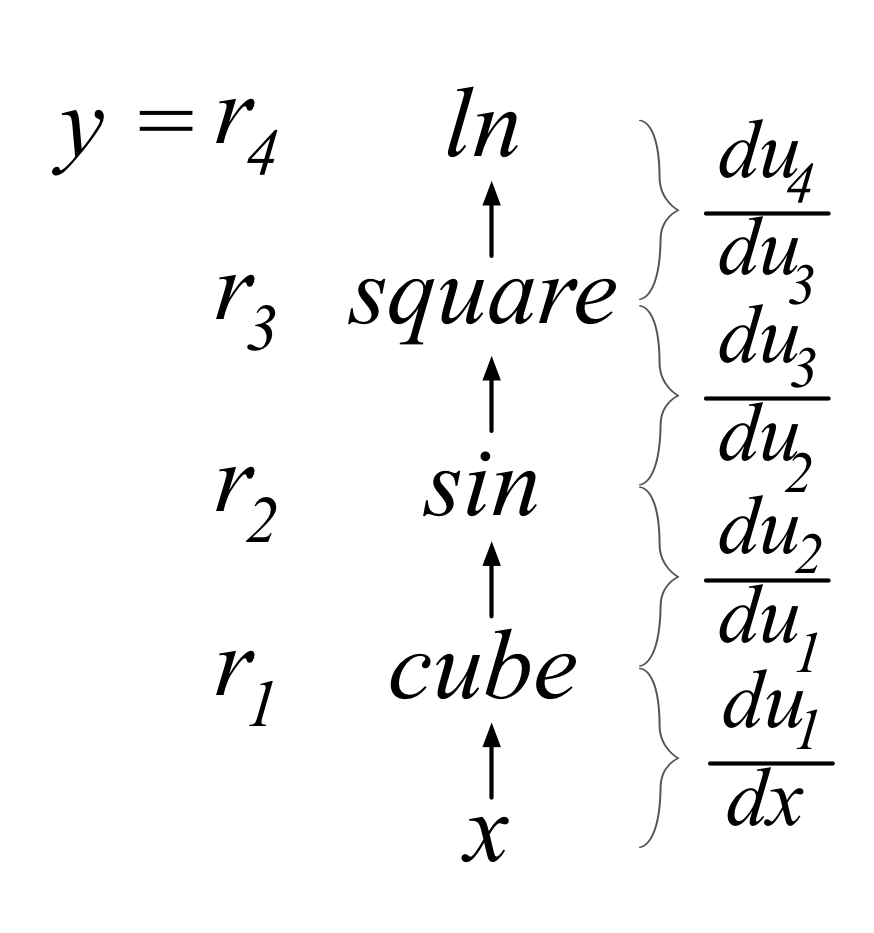
\includegraphics{chain-tree.png}
\end{center}

到目前为止,我们可以使用链式法则来求解单变量 $x$ 的嵌套表达式的导数,但仅当 $x$ 通过单一数据流路径影响 $y$ 时适用。要处理更复杂的表达式,我们需要扩展我们的技术,这将在下一节进行。


\subsubsection{单变量全导数链式法则}\label{sec4.5.2}

我们的单变量链式法则的应用范围有限,因为所有中间变量必须是单变量函数。但是,它展示了链式法则的核心机制,即乘以所有中间子表达式的导数。然而,要处理更一般的表达式,如 $y = f(x) = x + x^2$,我们需要增强这个基本的链式法则。

当然,我们立即可以看到 $\frac{dy}{dx} = \frac{d}{dx}x + \frac{d}{dx}x^2 = 1 + 2x$,但这使用的是标量加法导数规则,而不是链式法则。如果我们尝试应用单变量链式法则,我们会得到错误的答案。事实上,在这种情况下,之前的链式法则是没有意义的,因为导数算子 $\frac{d}{dx}$ 不适用于多元函数,例如我们中间变量中的 $u_2$:
\[
\begin{array}{lllllllll}
 u_1(x) &=& x^2\\
 u_2(x,u_1) &=& x + u_1 & & & (y = f(x) = u_2(x,u_1))
\end{array}
\]
我们试着应用一下,看看会发生什么。如果我们假装 $\frac{du_2}{du_1} = 0 + 1 = 1$ 和 $\frac{du_1}{dx} = 2x$,那么 $\frac{dy}{dx} = \frac{du_2}{dx} = \frac{du_2}{du_1} \frac{du_1}{dx} = 2x$,而不是正确的答案 $1 + 2x$。

因为 $u_2(x,u) = x + u_1$ 有多个参数,偏导数就派上用场了。我们盲目地对所有方程应用偏导数算子,看看会得到什么:
\[
\begin{array}{lllllllll}
 \frac{\partial u_1(x)}{\partial x} &=& 2x &&&(\text{与 }\frac{du_1(x)}{dx}\text{相同})\\
 \frac{\partial u_2(x,u_1)}{\partial u_1} &=& \frac{\partial }{\partial u_1}(x + u_1) = 0 + 1 = 1\\
 \frac{\partial u_2(x,u_1)}{\partial x} &
\includegraphics[scale=.012]{not-equal-icon.png}& \frac{\partial }{\partial x}(x + u_1) = 1 + 0 = 1 & & &(\text{这里有点不对劲!})
\end{array}
\]
哦不!偏导数 $\frac{\partial u_2(x,u_1)}{\partial x}$ 是错的,因为它违反了偏导数的一个关键假设。在对 $x$ 求偏导数时,其他变量必须不随 $x$ 变化。显然,$u_1(x) = x^2$ 是 $x$ 的函数,并且会随着 $x$ 变化。$\frac{\partial u_2(x,u_1)}{\partial x} \neq 1 + 0$ 因为 $\frac{\partial u_1(x)}{\partial x} \neq 0$。快速看一下 $y = u_2(x,u_1)$ 的数据流图,可以看到从 $x$ 到 $y$ 有多个路径,显然需要考虑 $x$ 的直接和间接(通过 $u_1(x)$)依赖:

\begin{center}
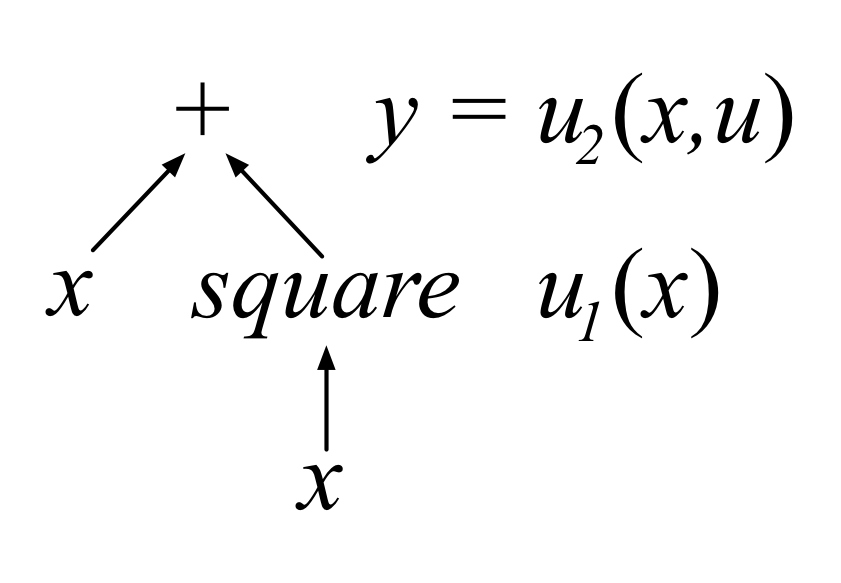
\includegraphics{plus-square.png}
\end{center}

$x$ 的变化会影响 $y$,既是加法的操作数,也是平方操作的操作数。以下方程描述了 $x$ 的微小变化如何影响输出:
\[\hat y = (x + \Delta x) + (x + \Delta x)^2\]
然后,$\Delta y = \hat y - y$,这可以理解为“$y$ 的变化是原始 $y$ 和 $x$ 调整后 $y$ 之间的差值”。

如果令 $x=1$,则 $y=1+1^2=2$。如果我们增加 $x$ 1,$\Delta x=1$,那么 $\hat y = (1+1) + (1+1)^2 = 2 + 4 = 6$。$y$ 的变化不是 1,如 $\partial u_2 / \partial u_1$ 所暗示的,而是 $6-2 = 4$!

引入“全导数”法则,基本上说,要计算 $\frac{dy}{dx}$,我们需要汇总所有可能的 $x$ 变化对 $y$ 变化的影响。关于 $x$ 的全导数假设所有变量,如本例中的 $u_1$,都是 $x$ 的函数,并且可能随 $x$ 变化。函数 $f(x) = u_2(x,u_1)$ 的全导数,它直接依赖于 $x$ 并通过中间变量 $u_1(x)$ 间接依赖,由下式给出:
\[\frac{dy}{dx} = \frac{\partial f(x)}{\partial x} = \frac{\partial u_2(x,u_1)}{\partial x} = \frac{\partial u_2}{\partial x}\frac{\partial x}{\partial x} + \frac{\partial u_2}{\partial u_1}\frac{\partial u_1}{\partial x} = \frac{\partial u_2}{\partial x} + \frac{\partial u_2}{\partial u_1}\frac{\partial u_1}{\partial x}\]
使用这个公式,我们得到正确的答案:
\[
\frac{dy}{dx} = \frac{\partial f(x)}{\partial x} = \frac{\partial u_2}{\partial x} + \frac{\partial u_2}{\partial u_1}\frac{\partial  u_1}{\partial  x} = 1 + 1 \times 2x = 1 + 2x
\]
这就是我们所谓的“单变量全导数链式法则”的应用:
\[
\frac{\partial f(x,u_1,\ldots,u_n)}{\partial x} = \frac{\partial f}{\partial x} + \frac{\partial f}{\partial u_1}\frac{\partial  u_1}{\partial  x} + \frac{\partial f}{\partial u_2}\frac{\partial  u_2}{\partial  x} + \ldots + \frac{\partial f}{\partial u_n}\frac{\partial  u_n}{\partial x} = \frac{\partial f}{\partial x} + \sum_{i=1}^n \frac{\partial f}{\partial u_i}\frac{\partial  u_i}{\partial  x}
\]
全导数假设所有变量可能相互依赖,而偏导数假设除 $x$ 以外的所有变量都是常数。

这里有一些微妙的记号问题。所有的导数都表示为偏导数,因为 $f$ 和 $u_i$ 是多变量函数。这种记号与 \href{http://mathworld.wolfram.com/TotalDerivative.html}{MathWorld 的记号} 一致,但与 \href{https://en.wikipedia.org/wiki/Total_derivative}{维基百科} 不同,维基百科使用 ${d f(x,u_1,\ldots,u_n)}/{d x}$(可能为了强调全导数的性质)。我们将继续使用偏导数记号,以便与下一节中向量链式法则的讨论保持一致。

实际应用中,只需记住,当你对 $x$ 求全导数时,其他变量可能是 $x$ 的函数,因此需要加上它们的贡献。方程的左边看起来像是典型的偏导数,但右边实际上是全导数。然而,通常许多临时变量是单个参数的函数,这意味着单变量全导数链式法则退化为单变量链式法则。

让我们来看一个嵌套子表达式,例如 $f(x) = \sin(x + x^2)$。我们引入三个中间变量:
\[
\begin{array}{lllllllll}
 u_1(x) &=& x^2\\
 u_2(x,u_1) &=& x + u_1\\
 u_3(u_2) &=& \sin(u_2) &&&(y = f(x) = u_3(u_2))
\end{array}
\]
以及偏导数:
\[
\begin{array}{lllllllll}
 \frac{\partial u_1}{\partial x} &=& 2x\\
 \frac{\partial u_2}{\partial x} &=& \frac{\partial x}{\partial x} + \frac{\partial u_2}{\partial u_1}\frac{\partial u_1}{\partial x} &=& 1 + 1 \times 2x &=& 1+2x\\
 \frac{\partial f(x)}{\partial x} &=& \frac{\partial u_3}{\partial x} + \frac{\partial u_3}{\partial u_2}\frac{\partial u_2}{\partial x} &=& 0 + \cos(u_2)\frac{\partial u_2}{\partial x} &=& \cos(x+x^2)(1+2x)
\end{array}
\]
其中,$\frac{\partial u_2}{\partial x}$ 和 $\frac{\partial f(x)}{\partial x}$ 都有 $\frac{\partial u_i}{\partial x}$ 项,考虑到了全导数。

还请注意,全导数公式总是“求和”,而不是,例如,乘以项 $\frac{\partial f}{\partial u_i}\frac{\partial  u_i}{\partial  x}$。可能有人会认为求和项在导数中是有意义的,例如,$y = x + x^2$ 添加了两个项。不完全是这样。全导数求和是因为它表示所有 $x$ 对 $y$ 变化贡献的加权和。例如,如果 $y = x \times x^2$ 而不是 $y = x + x^2$,全导数链式法则公式仍然添加偏导数项。($x \times x^2$ 简化为 $x^3$,但为了演示,我们不合并项。)以下是中间变量和偏导数:
\[
\begin{array}{lllllllll}
 u_1(x) &=& x^2\\
 u_2(x,u_1) &=& x u_1 &&& (y = f(x) = u_2(x,u_1))\\
\\
 \frac{\partial u_1}{\partial x} &=& 2x\\
 \frac{\partial u_2}{\partial x} &=& u_1 &&&(\text{对于 } u_2 = x + u_1, \frac{\partial u_2}{\partial x} = 1)\\
 \frac{\partial u_2}{\partial u_1} &=& x &&&(\text{对于 } u_2 = x + u_1, \frac{\partial u_2}{\partial u_1} = 1)
\end{array}
\]
全导数的形式仍然相同:
\[\frac{dy}{dx} = \frac{\partial u_2}{\partial x} + \frac{\partial u_2}{\partial u_1}\frac{d u_1}{\partial  x} = u_1 + x 2x = x^2 + 2x^2 = 3x^2\]
是偏导数(权重)改变了,而不是公式,当中间变量操作符改变时。

对于有较强微积分背景的读者,可能会 wondering 为什么我们即使对于非嵌套子表达式(如 $x^2$ 在 $x + x^2$ 中)也积极引入中间变量。我们使用这个过程有三个原因:(i) 计算简化的子表达式的导数通常是 trivia 的,(ii) 我们可以简化链式法则,(iii) 这个过程模仿了神经网络库中自动微分的工作方式。

更加积极地引入中间变量,让我们看看如何将单变量全导数链式法则简化为最终形式。目标是消除前面突出的 $\frac{\partial f}{\partial x}$:
\[
\frac{\partial f(x,u_1,\ldots,u_n)}{\partial x} = \frac{\partial f}{\partial x} + \sum_{i=1}^n \frac{\partial f}{\partial u_i}\frac{\partial  u_i}{\partial  x}
\]
我们可以通过简单地引入一个新的临时变量作为 $x$ 的别名来实现这一点:$u_{n+1} = x$。然后,公式简化为我们最终的形式:
\[
\frac{\partial f(u_1,\ldots,u_{n+1})}{\partial x} = \sum_{i=1}^{n+1} \frac{\partial f}{\partial u_i}\frac{\partial  u_i}{\partial  x}
\]
这个考虑全导数的链式法则退化为单变量链式法则,当所有中间变量都是单变量函数时。因此,你可以记住这个更一般的公式来覆盖两种情况。作为一个戏剧性的铺垫,注意求和看起来很像向量点积,$\frac{\partial f}{\partial \mathbf{u}} \cdot \frac{\partial \mathbf{u}}{\partial x}$,或者向量乘法 $\frac{\partial f}{\partial \mathbf{u}} \frac{\partial \mathbf{u}}{\partial x}$。

在继续之前,关于网上的术语,我要提醒一下。不幸的是,基于全导数的本节给出的链式法则在微积分讨论中普遍被称为“多元链式法则”,这非常具有误导性!只有中间变量是多元函数。总体函数,比如 $f(x) = x + x^2$,是接受单个参数 $x$ 的标量函数。导数和参数是标量,而不是向量,正如所谓的多元链式法则所预期的。为了减少混淆,我们使用“单变量全导数链式法则”来明确区分简单的单变量链式法则,$\frac{dy}{dx} = \frac{dy}{du}\frac{du}{dx}$,和这个法则。


\subsubsection{向量链式法则}\label{sec4.5.3}

现在我们对全导数链式法则有了很好的掌握,我们可以着手处理函数向量和向量变量的链式法则。令人惊讶的是,这个更一般的链式法则看起来和单变量标量的链式法则一样简单。我们不直接给出向量链式法则,而是通过自己重新发现它,以便更好地掌握它。我们可以从计算一个向量函数对标量的导数开始,例如
\[
\begin{bmatrix}
y_1(x)\\
y_2(x)\\
\end{bmatrix} =
\begin{bmatrix}
f_1(x)\\
f_2(x)\\
\end{bmatrix} = 
\begin{bmatrix}
\ln(x^2)\\
\sin(3x)
\end{bmatrix}
\]
看看能否抽象出一个通用公式。

我们引入两个中间变量 \(g_1\) 和 \(g_2\),每个 \(f_i\) 对应一个,使得 \(\mathbf{y}\) 看起来像 \(\mathbf{y} = \mathbf{f}(\mathbf{g}(x))\):
\[
\begin{bmatrix}
g_1(x)\\
g_2(x)\\
\end{bmatrix} = \begin{bmatrix}
x^2\\
3x\\
\end{bmatrix}
\]
\[
\begin{bmatrix}
f_1(\mathbf{g})\\
f_2(\mathbf{g})\\
\end{bmatrix} = \begin{bmatrix}
\ln(g_1)\\
\sin(g_2)\\
\end{bmatrix}
\]

向量 \(\mathbf{y}\) 对标量 \(x\) 的导数是一个垂直向量,其元素使用单变量全导数链式法则计算:
\[
\frac{\partial \mathbf{y}}{\partial x}  =
\begin{bmatrix}
\frac{\partial f_1(\mathbf{g})}{\partial x}\\
\frac{\partial f_2(\mathbf{g})}{\partial x}\\
\end{bmatrix} = \begin{bmatrix}
\frac{\partial f_1}{\partial g_1}\frac{\partial g_1}{\partial x} + \frac{\partial f_1}{\partial g_2}\frac{\partial g_2}{\partial x}\\
\frac{\partial f_2}{\partial g_1}\frac{\partial g_1}{\partial x} + \frac{\partial f_2}{\partial g_2}\frac{\partial g_2}{\partial x}\\
\end{bmatrix} = \begin{bmatrix}
\frac{1}{g_1}2x + 0\\
0 + \cos(g_2)3\\
\end{bmatrix} = \begin{bmatrix}
\frac{2x}{x^2}\\
3\cos(3x)\\
\end{bmatrix} = \begin{bmatrix}
\frac{2}{x}\\
3\cos(3x)\\
\end{bmatrix}
\]

我们得到了与标量方法相同的结果。这个向量链式法则对于函数向量和单个参数似乎是对的,确实与单变量链式法则相似。

如果我们把 \(\frac{\partial f_i}{\partial g_j}\frac{\partial g_j}{\partial x}\) 这些项分开,把 \(\frac{\partial g_j}{\partial x}\) 项隔离成一个向量,就得到一个矩阵与向量的乘积:
\[
\begin{bmatrix}
\frac{\partial f_1}{\partial g_1} & \frac{\partial f_1}{\partial g_2}\\
\frac{\partial f_2}{\partial g_1} & \frac{\partial f_2}{\partial g_2}\\
\end{bmatrix}
\begin{bmatrix}
\frac{\partial g_1}{\partial x}\\
\frac{\partial g_2}{\partial x}\\
\end{bmatrix} = \frac{\partial \mathbf{f}}{\partial \mathbf{g}}\frac{\partial \mathbf{g}}{\partial x}
\]

我们验证了结果:
\[
\frac{\partial \mathbf{f}}{\partial \mathbf{g}}\frac{\partial \mathbf{g}}{\partial x} = \begin{bmatrix}
\frac{1}{g_1} & 0\\
0 & \cos(g_2)\\
\end{bmatrix}
\begin{bmatrix}
2x\\
3\\
\end{bmatrix} = \begin{bmatrix}
\frac{1}{g_1}2x + 0\\
0 + \cos(g_2)3\\
\end{bmatrix} = \begin{bmatrix}
\frac{2}{x}\\
3\cos(3x)\\
\end{bmatrix}
\]

为了使这个公式适用于多个参数或向量 \(\mathbf{x}\),我们只需要将 \(x\) 换成向量 \(\mathbf{x}\)。此时,\(\frac{\partial \mathbf{g}}{\partial \mathbf{x}}\) 和 \(\frac{\partial \mathbf{f}}{\partial \mathbf{x}}\) 都变成了矩阵。我们的完整向量链式法则是:
\[
\frac{\partial}{\partial \mathbf{x}} \mathbf{f}(\mathbf{g}(\mathbf{x})) = \frac{\partial \mathbf{f}}{\partial \mathbf{g}}\frac{\partial \mathbf{g}}{\partial \mathbf{x}}
\]

完整的雅可比矩阵表示如下,其中 \(m=|\mathbf{f}|\),\(n=|\mathbf{x}|\),\(k=|\mathbf{g}|\)。结果的雅可比矩阵是 \(m \times n\)(一个 \(m \times k\) 矩阵乘以一个 \(k \times n\) 矩阵)。
\[
\frac{\partial}{\partial \mathbf{x}} \mathbf{f}(\mathbf{g}(\mathbf{x})) = \begin{bmatrix}
\frac{\partial f_1}{\partial g_1} & \frac{\partial f_1}{\partial g_2} & \ldots & \frac{\partial f_1}{\partial g_k}\\
\frac{\partial f_2}{\partial g_1} & \frac{\partial f_2}{\partial g_2} & \ldots & \frac{\partial f_2}{\partial g_k}\\
& &\ldots\\
\frac{\partial f_m}{\partial g_1} & \frac{\partial f_m}{\partial g_2} & \ldots & \frac{\partial f_m}{\partial g_k}\\
\end{bmatrix}
\begin{bmatrix}
\frac{\partial g_1}{\partial x_1} & \frac{\partial g_1}{\partial x_2} & \ldots & \frac{\partial g_1}{\partial x_n}\\
\frac{\partial g_2}{\partial x_1} & \frac{\partial g_2}{\partial x_2} & \ldots & \frac{\partial g_2}{\partial x_n}\\
& &\ldots\\
\frac{\partial g_k}{\partial x_1} & \frac{\partial g_k}{\partial x_2} & \ldots & \frac{\partial g_k}{\partial x_n}\\
\end{bmatrix}
\]

在这种情况下,向量链式法则简化为:
\[
\frac{\partial}{\partial \mathbf{x}} \mathbf{f}(\mathbf{g}(\mathbf{x})) = \text{diag}\left(\frac{\partial f_i}{\partial g_i}\right) \text{diag}\left(\frac{\partial g_i}{\partial x_i}\right) = \text{diag}\left(\frac{\partial f_i}{\partial g_i} \frac{\partial g_i}{\partial x_i}\right)
\]

最后,作者总结说只需要记住向量链式法则,因为单变量公式是其特例,并给出了一个表格来总结不同情况下的雅可比矩阵乘积。

\begin{center}
\begin{tabular}[t]{c|cccc}
  & 
\multicolumn{2}{c}{
  \begin{tabular}[t]{c}
  标量\\
  \framebox(18,18){$x$}\\
  \end{tabular}} & &\begin{tabular}{c}
  向量\\
  \framebox(18,40){$\mathbf{x}$}\\
  \end{tabular} \\
  
  \begin{tabular}{c}$\frac{\partial}{\partial \mathbf{x}} \mathbf{f}(\mathbf{g}(\mathbf{x}))$
	   = $\frac{\partial \mathbf{f}}{\partial \mathbf{g}}\frac{\partial\mathbf{g}}{\partial \mathbf{x}}$
		\\
		\end{tabular} & \begin{tabular}[t]{c}
  标量\\
  \framebox(18,18){$u$}\\
  \end{tabular} & \begin{tabular}{c}
  向量\\
  \framebox(18,40){$\mathbf{u}$}
  \end{tabular}& & \begin{tabular}{c}
  向量\\
  \framebox(18,40){$\mathbf{u}$}\\
  \end{tabular} \\
\hline
\\[\dimexpr-\normalbaselineskip+5pt]

\begin{tabular}[b]{c}
  标量\\
  \framebox(18,18){$f$}\\
  \end{tabular} &\framebox(18,18){$\frac{\partial f}{\partial {u}}$} \framebox(18,18){$\frac{\partial u}{\partial {x}}$} ~~~& \raisebox{22pt}{\framebox(40,18){$\frac{\partial f}{\partial {\mathbf{u}}}$}} \framebox(18,40){$\frac{\partial \mathbf{u}}{\partial x}$} & ~~~&
\raisebox{22pt}{\framebox(40,18){$\frac{\partial f}{\partial {\mathbf{u}}}$}} \framebox(40,40){$\frac{\partial \mathbf{u}}{\partial \mathbf{x}}$}
\\
  
\begin{tabular}[b]{c}
  向量\\
  \framebox(18,40){$\mathbf{f}$}\\
  \end{tabular} & \framebox(18,40){$\frac{\partial \mathbf{f}}{\partial {u}}$} \raisebox{22pt}{\framebox(18,18){$\frac{\partial u}{\partial {x}}$}} & \framebox(40,40){$\frac{\partial \mathbf{f}}{\partial \mathbf{u}}$} \framebox(18,40){$\frac{\partial \mathbf{u}}{\partial x}$} & & \framebox(40,40){$\frac{\partial \mathbf{f}}{\partial \mathbf{u}}$} \framebox(40,40){$\frac{\partial \mathbf{u}}{\partial \mathbf{x}}$}\\
  
\end{tabular}
\end{center}

\section{神经元激活的梯度}\label{sec5}

我们现在有了所有需要的部件,可以计算典型神经元激活对于单个神经网络计算单元的模型参数 $\mathbf{w}$ 和 $b$ 的导数:
\[ \text{activation}(\mathbf{x}) = \max(0, \mathbf{w} \cdot \mathbf{x} + b) \]
(这表示一个具有全连接权重和修正线性单元激活的神经元。不过,还有其他的仿射函数,如卷积,以及其他激活函数,如指数线性单元,其逻辑类似。)

我们先不考虑 $\max$,而是专注于计算 $\frac{\partial}{\partial \mathbf{w}} (\mathbf{w} \cdot \mathbf{x} + b)$ 和 $\frac{\partial}{\partial b} (\mathbf{w} \cdot \mathbf{x} + b)$。(回想一下,神经网络通过优化权重和偏置来进行学习。)我们还没有讨论点积的导数,$y = \mathbf{f(w)} \cdot \mathbf{g(x)}$,但可以使用链式法则来避免记忆另一个规则。(注意符号 $y$ 而不是 $\mathbf{y}$,因为结果是一个标量而不是向量。)

点积 $\mathbf{w} \cdot \mathbf{x}$ 只是元素-wise 乘积的求和:$\sum_{i=1}^n (w_i x_i) = \text{sum}(\mathbf{w} \otimes \mathbf{x})$。(你可能还发现记住线性代数符号 $\mathbf{w} \cdot \mathbf{x} = \mathbf{w}^{T} \mathbf{x}$ 会很有用。)我们知道如何计算 $\text{sum}(\mathbf{x})$ 和 $\mathbf{w} \otimes \mathbf{x}$ 的偏导数,但还没有研究过 $\text{sum}(\mathbf{w} \otimes \mathbf{x})$ 的偏导数。为此我们需要链式法则,并且可以引入一个中间向量变量 $\mathbf{u}$,就像我们使用单变量链式法则时所做的那样:
\[
\begin{array}{lllllllll}
 \mathbf{u} &=& \mathbf{w} \otimes \mathbf{x} \\
 y &=& \text{sum}(\mathbf{u}) \\
\end{array}
\]
一旦我们重新表述了 $y$,就识别出两个子表达式,其偏导数我们已经知道:
\[
\begin{array}{lllllllll}
 \frac{\partial \mathbf{u}}{\partial \mathbf{w}} &=& \frac{\partial }{\partial \mathbf{w}} (\mathbf{w} \otimes \mathbf{x}) &=& \text{diag}(\mathbf{x}) \\
 \frac{\partial y}{\partial \mathbf{u}} &=& \frac{\partial }{\partial \mathbf{u}} \text{sum}(\mathbf{u}) &=& \vec{1}^T \\
\end{array}
\]
向量链式法则说要乘以偏导数:
\[\frac{\partial y}{\partial \mathbf{w}} = \frac{\partial y}{\partial \mathbf{u}} \frac{\partial \mathbf{u}}{\partial \mathbf{w}} = \vec{1}^T \text{diag}(\mathbf{x}) = \mathbf{x}^T\]
为了验证我们的结果,我们可以将点积分解为纯标量函数:
\[
\begin{array}{lllllllll}
 y &=& \mathbf{w} \cdot \mathbf{x} &=& \sum_{i=1}^n (w_i x_i) \\
 \frac{\partial y}{\partial w_j} &=& \frac{\partial}{\partial w_j} \sum_i (w_i x_i) &=& \sum_i \frac{\partial}{\partial w_j} (w_i x_i) &=& \frac{\partial}{\partial w_j} (w_j x_j) &=& x_j \\
\end{array}
\]
然后:
\[\frac{\partial y}{\partial \mathbf{w}} = [ x_1, \ldots, x_n ] = \mathbf{x}^T\]
太好了!我们的标量结果与向量链式法则结果一致。

现在,令 $y = \mathbf{w} \cdot \mathbf{x} + b$,即 $max$ 激活函数调用内的完整表达式。我们需要计算两个不同的偏导数,但不需要链式法则:
\[
\begin{array}{lllllllll}
 \frac{\partial y}{\partial \mathbf{w}} &=& \frac{\partial }{\partial \mathbf{w}} \mathbf{w} \cdot \mathbf{x} + \frac{\partial }{\partial \mathbf{w}} b &=& \mathbf{x}^T + \vec{0}^T &=& \mathbf{x}^T \\
 \frac{\partial y}{\partial b} &=& \frac{\partial }{\partial b} \mathbf{w} \cdot \mathbf{x} + \frac{\partial }{\partial b} b &=& 0 + 1 &=& 1 \\
\end{array}
\]
现在我们来计算神经元激活 $max(0, \mathbf{w} \cdot \mathbf{x} + b)$ 的偏导数。使用标量 $z$ 上的 $max(0,z)$ 函数调用,意思是将所有负的 $z$ 值视为 0。$max$ 函数的导数是一个分段函数。当 $z \leq 0$ 时,导数为 0,因为 $z$ 是常数。当 $z > 0$ 时,$max$ 函数的导数就是 $z$ 的导数,即 $1$:
\[ \frac{\partial}{\partial z} \max(0,z) =
	\begin{cases}
	0 & z \leq 0 \\
	\frac{dz}{dz}=1 & z > 0
	\end{cases}
\]
关于将函数广播到标量的附带说明。当$max$的其中一个或两个参数是向量时,例如 $max(0,\mathbf{x})$,我们将单变量函数 $max$ 广播到元素上。这是一个逐元素一元运算符的例子。为了明确起见:
\[
\max(0,\mathbf{x}) = \begin{bmatrix}
 \max(0,x_1) \\
 \max(0,x_2) \\
 \ldots \\
 \max(0,x_n)
\end{bmatrix}
\]
对于广播版本的导数,我们得到一个由 0 和 1 组成的向量:
\[
\frac{\partial}{\partial x_i} \max(0,x_i) =
	\begin{cases}
	0 & x_i \leq 0 \\
	\frac{dx_i}{dx_i}=1 & x_i > 0
	\end{cases}
\]
\[\frac{\partial}{\partial \mathbf{x}} \max(0,\mathbf{x}) =
\begin{bmatrix}
	\frac{\partial}{\partial x_1} \max(0,x_1) \\
	\frac{\partial}{\partial x_2} \max(0,x_2) \\
	\ldots \\
    \frac{\partial}{\partial x_n} \max(0,x_n)
\end{bmatrix}
\]
为了得到激活函数 $activation(\mathbf{x})$ 的导数,我们需要链式法则,因为有嵌套的子表达式 $\mathbf{w} \cdot \mathbf{x} + b$。按照我们的过程,引入中间标量变量 $z$ 来表示仿射函数:
\[ z(\mathbf{w},b,\mathbf{x}) = \mathbf{w} \cdot \mathbf{x} + b \]
\[ activation(z) = \max(0,z) \]
向量链式法则告诉我们:
\[\frac{\partial activation}{\partial \mathbf{w}} = \frac{\partial activation}{\partial z} \frac{\partial z}{\partial \mathbf{w}}\]
可以重写为:
\[\frac{\partial activation}{\partial \mathbf{w}} = \begin{cases}
	0 \frac{\partial z}{\partial \mathbf{w}} = \vec{0}^T & z \leq 0 \\
	1 \frac{\partial z}{\partial \mathbf{w}} = \frac{\partial z}{\partial \mathbf{w}} = \mathbf{x}^T & z > 0 \quad (\text{我们之前计算过 } \frac{\partial z}{\partial \mathbf{w}} = \mathbf{x}^T) \\
\end{cases}\]
然后代入 $z = \mathbf{w} \cdot \mathbf{x} + b$:
\[\frac{\partial activation}{\partial \mathbf{w}} = \begin{cases}
	\vec{0}^T & \mathbf{w} \cdot \mathbf{x} + b \leq 0 \\
	\mathbf{x}^T & \mathbf{w} \cdot \mathbf{x} + b > 0
\end{cases}\]
这个方程符合我们的直觉。当激活函数将仿射函数输出 $z$ 截断为 0 时,关于任何权重 $w_i$ 的导数为零。当 $z > 0$ 时,好像 $max$ 函数消失了,我们只得到 $z$ 关于权重的导数。

接下来是神经元激活关于 $b$ 的导数:
\[\frac{\partial activation}{\partial b} = \begin{cases}
	0 \frac{\partial z}{\partial b} = 0 & \mathbf{w} \cdot \mathbf{x} + b \leq 0 \\
	1 \frac{\partial z}{\partial b} = 1 & \mathbf{w} \cdot \mathbf{x} + b > 0
\end{cases}\]
现在,我们使用这些偏导数来处理整个损失函数。


\section{神经网络损失函数的梯度}\label{sec6}

训练神经元需要我们对损失函数或“代价”函数关于模型的参数 $\mathbf{w}$ 和 $b$ 求导。因为我们用多个向量输入(例如,多张图像)和标量目标(例如,每张图像一个分类)进行训练,所以我们需要一些额外的符号。设
\[ X = [\mathbf{x}_1, \mathbf{x}_2, \ldots, \mathbf{x}_N]^T \]
其中 $N=|X|$,然后设
\[ \mathbf{y} = [\text{target}(\mathbf{x}_1), \text{target}(\mathbf{x}_2), \ldots, \text{target}(\mathbf{x}_N)]^T \]
其中 $y_i$ 是一个标量。于是代价方程变为:
\[ C(\mathbf{w},b,X,\mathbf{y}) = \frac{1}{N} \sum_{i=1}^{N} (y_i - \text{activation}(\mathbf{x}_i))^2 = \frac{1}{N} \sum_{i=1}^{N} (y_i - \max(0, \mathbf{w}\cdot\mathbf{x}_i+b))^2 \]
按照我们的链式法则过程,引入这些中间变量:
\[
\begin{array}{lllllllll} 
 u(\mathbf{w},b,\mathbf{x}) &=& \max(0, \mathbf{w}\cdot\mathbf{x}+b)\\
 v(y,u) &=& y - u\\
 C(v) &=& \frac{1}{N} \sum_{i=1}^N v^2\\
\end{array}
\]
首先我们来计算关于 $\mathbf{w}$ 的梯度。

\subsection{关于权重的梯度}\label{sec6.1}

之前我们知道:
\[\frac{\partial }{\partial \mathbf{w}} u(\mathbf{w},b,\mathbf{x}) = \begin{cases}
	\vec{0}^T & \mathbf{w} \cdot \mathbf{x} + b \leq 0\\
	\mathbf{x}^T & \mathbf{w} \cdot \mathbf{x} + b > 0\\
\end{cases}\]
和
\[\frac{\partial v(y,u)}{\partial \mathbf{w}} = \frac{\partial}{\partial \mathbf{w}} (y - u) = \vec{0}^T - \frac{\partial u}{\partial \mathbf{w}} = -\frac{\partial u}{\partial \mathbf{w}} = \begin{cases}
	\vec{0}^T & \mathbf{w} \cdot \mathbf{x} + b \leq 0\\
	-\mathbf{x}^T & \mathbf{w} \cdot \mathbf{x} + b > 0\\
\end{cases}\]
然后,对于整体梯度,我们得到:
\begin{center}
\begin{eqnarray*}
 \frac{\partial C(v)}{\partial \mathbf{w}} & = & \frac{\partial }{\partial \mathbf{w}}\frac{1}{N} \sum_{i=1}^N v^2\\\\
 & = & \frac{1}{N} \sum_{i=1}^N \frac{\partial}{\partial \mathbf{w}} v^2\\\\
 & = & \frac{1}{N} \sum_{i=1}^N \frac{\partial v^2}{\partial v} \frac{\partial v}{\partial \mathbf{w}} \\\\
 & = & \frac{1}{N} \sum_{i=1}^N 2v \frac{\partial v}{\partial \mathbf{w}} \\\\
 & = & \frac{1}{N} \sum_{i=1}^N \begin{cases}
	2v\vec{0}^T = \vec{0}^T & \mathbf{w} \cdot \mathbf{x}_i + b \leq 0\\
	-2v\mathbf{x}^T & \mathbf{w} \cdot \mathbf{x}_i + b > 0\\
\end{cases}\\\\
 & = & \frac{1}{N} \sum_{i=1}^N \begin{cases}
	\vec{0}^T & \mathbf{w} \cdot \mathbf{x}_i + b \leq 0\\
	-2(y_i-u)\mathbf{x}_i^T & \mathbf{w} \cdot \mathbf{x}_i + b > 0\\
\end{cases}\\\\
 & = & \frac{1}{N} \sum_{i=1}^N \begin{cases}
	\vec{0}^T & \mathbf{w} \cdot \mathbf{x}_i + b \leq 0\\
	-2(y_i-\max(0, \mathbf{w}\cdot\mathbf{x}_i+b))\mathbf{x}_i^T & \mathbf{w} \cdot \mathbf{x}_i + b > 0\\
\end{cases}\\\\
 & = & \begin{cases}
	\vec{0}^T & \mathbf{w} \cdot \mathbf{x}_i + b \leq 0\\
	\frac{-2}{N} \sum_{i=1}^N (y_i-(\mathbf{w}\cdot\mathbf{x}_i+b))\mathbf{x}_i^T & \mathbf{w} \cdot \mathbf{x}_i + b > 0\\
\end{cases}\\\\
 & = & \begin{cases}
	\vec{0}^T & \mathbf{w} \cdot \mathbf{x}_i + b \leq 0\\
	\frac{2}{N} \sum_{i=1}^N (\mathbf{w}\cdot\mathbf{x}_i+b-y_i)\mathbf{x}_i^T & \mathbf{w} \cdot \mathbf{x}_i + b > 0\\
\end{cases}
\end{eqnarray*}
\end{center}
为了理解这个方程,我们可以引入误差项 $e_i = \mathbf{w}\cdot\mathbf{x}_i+b-y_i$,得到:
\[
\frac{\partial C}{\partial \mathbf{w}} = \frac{2}{N} \sum_{i=1}^N e_i\mathbf{x}_i^T \quad \text{(对于激活非零的情况)}
\]
从此可以看出,这个计算是对所有 $\mathbf{x}_i$ 在 $X$ 上的加权平均。权重是误差项,即每个输入 $\mathbf{x}_i$ 的目标输出和实际神经元输出之间的差值。梯度的平均值将指向更高的代价或损失方向,因为大的 $e_i$ 强调了其对应的 $\mathbf{x}_i$。想象我们只有一个输入向量,$N=|X|=1$,那么梯度就是 $2e_1\mathbf{x}_1^T$。如果误差为 0,则梯度为零,我们达到了最小损失。如果 $e_1$ 是某个小的正差值,梯度是在 $\mathbf{x}_1$ 方向上的一个小步。如果 $e_1$ 很大,梯度是一个大的步长。如果 $e_1$ 为负,则梯度方向相反,意味着最高的代价在负方向。

当然,我们希望减少而不是增加损失,这就是为什么梯度下降的递推关系取梯度的负方向来更新当前位置(对于标量学习率 $\eta$):
\[ \mathbf{w}_{t+1} = \mathbf{w}_{t} - \eta \frac{\partial C}{\partial \mathbf{w}} \]
因为梯度指示的是代价更高的方向,所以我们希望在相反的方向上更新 $\mathbf{w}$。

\subsection{关于偏置的导数}\label{sec6.2}

为了优化偏置 $b$,我们也需要关于 $b$ 的偏导数。以下是中间变量的定义:
\[
\begin{array}{lllllllll}
 u(\mathbf{w},b,\mathbf{x}) &=& \max(0, \mathbf{w}\cdot\mathbf{x}+b)\\
 v(y,u) &=& y - u\\
 C(v) &=& \frac{1}{N} \sum_{i=1}^N v^2\\
\end{array}
\]
我们之前计算过关于偏置的偏导数:
\[\frac{\partial u}{\partial b} = \begin{cases}
	0 & \mathbf{w} \cdot \mathbf{x} + b \leq 0\\
	1 & \mathbf{w} \cdot \mathbf{x} + b > 0\\
\end{cases}\]
对于 $v$,偏导数是:
\[\frac{\partial v(y,u)}{\partial b} = \frac{\partial}{\partial b} (y - u) = 0 - \frac{\partial u}{\partial b} = -\frac{\partial u}{\partial b} = \begin{cases}
	0 & \mathbf{w} \cdot \mathbf{x} + b \leq 0\\
	-1 & \mathbf{w} \cdot \mathbf{x} + b > 0\\
\end{cases}\]
对于代价函数本身的偏导数,我们得到:
\begin{center}
\begin{eqnarray*}
 \frac{\partial C(v)}{\partial b} & = & \frac{\partial }{\partial b}\frac{1}{N} \sum_{i=1}^N v^2\\\\
 & = & \frac{1}{N} \sum_{i=1}^N \frac{\partial}{\partial b} v^2\\\\
 & = & \frac{1}{N} \sum_{i=1}^N \frac{\partial v^2}{\partial v} \frac{\partial v}{\partial b} \\\\
 & = & \frac{1}{N} \sum_{i=1}^N 2v \frac{\partial v}{\partial b} \\\\
 & = & \frac{1}{N} \sum_{i=1}^N \begin{cases}
 	0 & \mathbf{w} \cdot \mathbf{x} + b \leq 0\\
 	-2v & \mathbf{w} \cdot \mathbf{x} + b > 0\\
 \end{cases}\\\\
 & = & \frac{1}{N} \sum_{i=1}^N \begin{cases}
 	0 & \mathbf{w} \cdot \mathbf{x} + b \leq 0\\
 	-2(y_i-\max(0, \mathbf{w}\cdot\mathbf{x}_i+b)) & \mathbf{w} \cdot \mathbf{x} + b > 0\\
 \end{cases}\\\\
 & = & \frac{1}{N} \sum_{i=1}^N \begin{cases}
 	0 & \mathbf{w} \cdot \mathbf{x} + b \leq 0\\
 	2(\mathbf{w}\cdot\mathbf{x}_i+b-y_i) & \mathbf{w} \cdot \mathbf{x} + b > 0\\
 \end{cases}\\\\
 & = & \begin{cases}
	0 & \mathbf{w} \cdot \mathbf{x}_i + b \leq 0\\
	\frac{2}{N} \sum_{i=1}^N (\mathbf{w}\cdot\mathbf{x}_i+b-y_i) & \mathbf{w} \cdot \mathbf{x}_i + b > 0\\
 \end{cases}
\end{eqnarray*}
\end{center}
同样地,我们可以引入误差项:
\[ \frac{\partial C}{\partial b} = \frac{2}{N} \sum_{i=1}^N e_i \quad \text{(对于激活非零的情况)} \]
偏导数就是平均误差或零,根据激活水平而定。为了更新神经元的偏置,我们将其朝减少代价的方向调整:
\[ b_{t+1} = b_{t} - \eta \frac{\partial C}{\partial b} \]
在实际应用中,将 $\mathbf{w}$ 和 $b$ 合并成一个单一的向量参数会更方便,而不是分别处理两个偏导数:$\hat{\mathbf{w}} = [\mathbf{w}^T, b]^T$。这需要对输入向量 $\mathbf{x}$ 也做相应的调整,但简化了激活函数。通过在 $\mathbf{x}$ 的末尾添加一个 1,即 $\hat{\mathbf{x}} = [\mathbf{x}^T,1]$,$\mathbf{w} \cdot \mathbf{x} + b$ 就变成了 $\hat{\mathbf{w}} \cdot \hat{\mathbf{x}}$。

这完成了神经网络损失函数的优化,因为我们已经得到了两个必要的偏导数来进行梯度下降。


\section{总结}\label{sec7}

希望您已经一路读到这里。您已经走在理解矩阵微积分的路上了!我们在下一节中包含了一个参考文献,总结了本文中所有规则。另外,请查看下面的注释资源链接。

您的下一步是学习矩阵的偏导数,而不仅仅是向量的偏导数。例如,您可以查阅 \href{https://atmos.washington.edu/~dennis/MatrixCalculus.pdf}{矩阵微积分} 中的矩阵微分部分。

{\bf 致谢}. 我们感谢 \href{https://www.usfca.edu/faculty/yannet-interian}{Yannet Interian}(美国圣弗朗西斯科大学数据科学硕士项目的教师)和 \href{http://www.cs.usfca.edu/~duminsky/}{David Uminsky}(数据科学硕士项目的教师兼主任),感谢他们在此处所呈现的符号表示方面的帮助。


\section{矩阵微积分参考}\label{reference}


\subsection{梯度和雅可比矩阵}\label{sec8.1}

二元函数的梯度是一个水平的2-向量:
\[
\nabla f(x,y)  = \left[ \frac{\partial f(x,y)}{\partial x}, \frac{\partial f(x,y)}{\partial y} \right]
\]
向量值函数关于向量的雅可比矩阵是一个$m \times n$矩阵(其中$m=|\mathbf{f}|$和$n=|\mathbf{x}|$),包含所有可能的标量偏导数:
\[
\frac{\partial \mathbf{y}}{\partial \mathbf{x}} = 
\begin{bmatrix}
\nabla f_1(\mathbf{x}) \\
\nabla f_2(\mathbf{x})\\
\vdots\\
\nabla f_m(\mathbf{x})
\end{bmatrix} = 
\begin{bmatrix}
\frac{\partial}{\partial \mathbf{x}} f_1(\mathbf{x}) \\
\frac{\partial}{\partial \mathbf{x}} f_2(\mathbf{x})\\
\vdots\\
\frac{\partial}{\partial \mathbf{x}} f_m(\mathbf{x})
\end{bmatrix} = 
\begin{bmatrix}
\frac{\partial}{\partial x_1} f_1(\mathbf{x}) & \frac{\partial}{\partial x_2} f_1(\mathbf{x}) & \cdots & \frac{\partial}{\partial x_n} f_1(\mathbf{x}) \\
\frac{\partial}{\partial x_1} f_2(\mathbf{x}) & \frac{\partial}{\partial x_2} f_2(\mathbf{x}) & \cdots & \frac{\partial}{\partial x_n} f_2(\mathbf{x}) \\
\vdots & \vdots & & \vdots \\
\frac{\partial}{\partial x_1} f_m(\mathbf{x}) & \frac{\partial}{\partial x_2} f_m(\mathbf{x}) & \cdots & \frac{\partial}{\partial x_n} f_m(\mathbf{x})
\end{bmatrix}
\]
恒等函数$\mathbf{f(x)} = \mathbf{x}$的雅可比矩阵是$I$。


\subsection{向量的逐元素运算}\label{sec8.2}

定义向量 $\mathbf{w}$ 和 $\mathbf{x}$ 上的通用逐元素运算,使用运算符 $\bigcirc$,例如 $+$:
\[
\begin{bmatrix}
           y_1\\
           y_2\\
           \vdots \\
           y_n\\
           \end{bmatrix} = \begin{bmatrix}
           f_{1}(\mathbf{w}) \bigcirc g_{1}(\mathbf{x})\\
           f_{2}(\mathbf{w}) \bigcirc g_{2}(\mathbf{x})\\
           \vdots \\
           f_{n}(\mathbf{w}) \bigcirc g_{n}(\mathbf{x})\\
         \end{bmatrix}
\]
关于 $\mathbf{w}$ 的雅可比矩阵(关于 $\mathbf{x}$ 类似)为:
\[ J_\mathbf{w} = 
\frac{\partial \mathbf{y}}{\partial \mathbf{w}}  = \begin{bmatrix}
\frac{\partial}{\partial w_1} ( f_{1}(\mathbf{w}) \bigcirc g_{1}(\mathbf{x}) ) & \frac{\partial}{\partial w_2} ( f_{1}(\mathbf{w}) \bigcirc g_{1}(\mathbf{x}) ) & \ldots & \frac{\partial}{\partial w_n} ( f_{1}(\mathbf{w}) \bigcirc g_{1}(\mathbf{x}) )\\
\frac{\partial}{\partial w_1} ( f_{2}(\mathbf{w}) \bigcirc g_{2}(\mathbf{x}) ) & \frac{\partial}{\partial w_2} ( f_{2}(\mathbf{w}) \bigcirc g_{2}(\mathbf{x}) ) & \ldots & \frac{\partial}{\partial w_n} ( f_{2}(\mathbf{w}) \bigcirc g_{2}(\mathbf{x}) )\\
& \ldots\\
\frac{\partial}{\partial w_1} ( f_{n}(\mathbf{w}) \bigcirc g_{n}(\mathbf{x}) ) & \frac{\partial}{\partial w_2} ( f_{n}(\mathbf{w}) \bigcirc g_{n}(\mathbf{x}) ) & \ldots & \frac{\partial}{\partial w_n} ( f_{n}(\mathbf{w}) \bigcirc g_{n}(\mathbf{x}) )\\
\end{bmatrix} 
\]
在约束条件(逐元素对角条件)下,即 $f_i(\mathbf{w})$ 和 $g_i(\mathbf{x})$ 最多访问 $w_i$ 和 $x_i$,雅可比矩阵简化为对角矩阵:
\[
\frac{\partial \mathbf{y}}{\partial \mathbf{w}} = diag \left( \frac{\partial}{\partial w_1}(f_{1}(w_1) \bigcirc g_{1}(x_1)),~ \frac{\partial}{\partial w_2}(f_{2}(w_2) \bigcirc g_{2}(x_2)),~ \ldots,~ \frac{\partial}{\partial w_n}(f_{n}(w_n) \bigcirc g_{n}(x_n)) \right)
\]
以下是一些逐元素运算的示例:
\[
\begin{array}{lll}
 \text{\bf 运算} & \text{\bf 关于 } \mathbf{w} \text{ 的偏导数} & \text{\bf 关于 } \mathbf{x} \text{ 的偏导数}\\
 + & \frac{\partial (\mathbf{w}+\mathbf{x})}{\partial \mathbf{w}} = I & \frac{\partial (\mathbf{w}+\mathbf{x})}{\partial \mathbf{x}} =  I\\
 - & \frac{\partial (\mathbf{w}-\mathbf{x})}{\partial \mathbf{w}}  = I & \frac{\partial (\mathbf{w}-\mathbf{x})}{\partial \mathbf{x}}  = -I \\
 \otimes & \frac{\partial (\mathbf{w} \otimes \mathbf{x})}{\partial \mathbf{w}}  =  diag(\mathbf{x}) & \frac{\partial (\mathbf{w} \otimes \mathbf{x})}{\partial \mathbf{x}}  =  diag(\mathbf{w})\\
 \oslash & \frac{\partial (\mathbf{w} \oslash \mathbf{x})}{\partial \mathbf{w}}  =  diag(\ldots \frac{1}{x_i} \ldots) & \frac{\partial (\mathbf{w} \oslash \mathbf{x})}{\partial \mathbf{x}}  =  diag(\ldots \frac{-w_i}{x_i^2} \ldots)\\
\end{array}
\]

\subsection{标量扩展}\label{sec8.3}

将标量 $z$ 加到向量 $\mathbf{x}$ 上,即 $\mathbf{y} = \mathbf{x} + z$,实际上是 $\mathbf{y} = \mathbf{f(x)} + \mathbf{g}(z)$,其中 $\mathbf{f(x)} = \mathbf{x}$ 和 $\mathbf{g}(z) = \vec{1} z$。
\[
\frac{\partial}{\partial \mathbf{x}} ( \mathbf{x} + z ) = diag(\vec{1}) = I
\]
\[
\frac{\partial}{\partial z} ( \mathbf{x} + z ) = \vec{1}
\]
标量乘法给出:
\[
\frac{\partial}{\partial \mathbf{x}} ( \mathbf{x} z ) = I z
\]
\[
\frac{\partial}{\partial z} ( \mathbf{x} z ) = \mathbf{x}
\]

\subsection{向量约简}\label{sec8.4}

一个向量和关于其中一个向量的偏导数为:
\[
\nabla_{\mathbf{x}} y = \begin{array}{lcl}
 \frac{\partial y}{\partial \mathbf{x}} & = & \begin{bmatrix} \frac{\partial y}{\partial x_1}, \frac{\partial y}{\partial x_2}, \ldots, \frac{\partial y}{\partial x_n} \end{bmatrix} = \begin{bmatrix} \sum_i \frac{\partial f_i(\mathbf{x})}{\partial x_1},~ \sum_i \frac{\partial f_i(\mathbf{x})}{\partial x_2},~ \ldots,~ \sum_i \frac{\partial f_i(\mathbf{x})}{\partial x_n}  \end{bmatrix}\\
\end{array}
\]
对于 $y = \text{sum}(\mathbf{x})$:
\[\nabla_\mathbf{x} y = \vec{1}^T\]
对于 $y = \text{sum}(\mathbf{x}z)$ 且 $n = |\mathbf{x}|$,我们得到:
\[\nabla_\mathbf{x} y = [z, z, \ldots, z]\]
\[\nabla_z y = \text{sum}(\mathbf{x}) \]
向量点积 $y = \mathbf{f(w)} \cdot \mathbf{g(x)} = \sum_{i=1}^n (w_i x_i) = \text{sum}(\mathbf{w} \otimes \mathbf{x})$。令 $\mathbf{u} = \mathbf{w} \otimes \mathbf{x}$ 并使用向量链式法则,我们得到:
\[
\begin{array}{lcl}
 \frac{d \mathbf{u}}{d\mathbf{x}} = \frac{d}{d\mathbf{x}} (\mathbf{w} \otimes \mathbf{x}) = \text{diag}(\mathbf{w})\\
 \frac{dy}{d\mathbf{u}} = \frac{d}{d\mathbf{u}} \text{sum}(\mathbf{u}) = \vec{1}^T\\
 \frac{dy}{d\mathbf{x}} = \frac{dy}{d\mathbf{u}} \times \frac{d\mathbf{u}}{d\mathbf{x}} = \vec{1}^T \times \text{diag}(\mathbf{w}) = \mathbf{w}^T
\end{array}
\]
类似地,$\frac{dy}{d\mathbf{w}} = \mathbf{x}^T$。

\subsection{链式法则}\label{sec8.5}

向量链式法则是其一般形式,因为它退化为其他形式。当 $f$ 是单变量 $x$ 的函数,并且所有中间变量 $u$ 都是单变量的函数时,单变量链式法则适用。当部分或全部中间变量是多变量函数时,单变量全导数链式法则适用。在其他所有情况下,适用向量链式法则。

\begin{tabular}{lll}
{\bf 单变量法则} & {\bf 单变量全导数法则} & {\bf 向量法则} \\
$\frac{df}{dx} = \frac{df}{du}\frac{du}{dx}$ & $\frac{\partial f(u_1,\ldots,u_n)}{\partial x} = \frac{\partial f}{\partial \mathbf{u}} \frac{\partial \mathbf{u}}{\partial x}$ & $\frac{\partial}{\partial \mathbf{x}} \mathbf{f}(\mathbf{g}(\mathbf{x})) = \frac{\partial \mathbf{f}}{\partial \mathbf{g}}\frac{\partial\mathbf{g}}{\partial \mathbf{x}}$ \\
\end{tabular}


\section{符号表}\label{notation}

斜体表示的黑体小写字母,如 $\mathbf{x}$,表示向量,而斜体小写字母,如 $x$,表示标量。$x_i$ 是向量 $\mathbf{x}$ 的第 $i$ 个元素,且为斜体,因为单个向量元素是标量。$|\mathbf{x}|$ 表示向量 $\mathbf{x}$ 的长度。

$\mathbf{x}^T$ 中的指数 $T$ 表示相应向量的转置。

$\sum_{i=a}^b x_i$ 表示一个从 $a$ 到 $b$ 对 $x_i$ 求和的 for 循环。

符号 $f(x)$ 表示一个以 $x$ 为参数的函数 $f$。

$I$ 表示适当维度的单位矩阵,其非对角线元素均为零,而对角线元素均为 1。

$diag(\mathbf{x})$ 表示一个以向量 $\mathbf{x}$ 的元素为对角线元素的矩阵。

点积 $\mathbf{w} \cdot \mathbf{x}$ 表示元素对应相乘后再求和,即 $\sum_i^n (w_i x_i) = sum(\mathbf{w} \otimes \mathbf{x})$。也可以看作 $w^T x$。

微分 $\frac{d}{dx}$ 是一个将单参数函数映射到另一个函数的算子。也就是说,$\frac{d}{dx} f(x)$ 将 $f(x)$ 映射到它关于 $x$ 的导数,这与 $\frac{df(x)}{dx}$ 是同一个意思。另外,如果 $y = f(x)$,那么 $\frac{dy}{dx} = \frac{df(x)}{dx} = \frac{d}{dx}f(x)$。

函数关于 $x$ 的偏导数 $\frac{\partial}{\partial x} f(x)$,执行的是保持其他变量不变的标量导数。

函数 $f$ 关于向量 $\mathbf{x}$ 的梯度 $\nabla f(\mathbf{x})$,组织了特定标量函数的所有偏导数。

雅可比矩阵组织了多个函数的梯度,并将它们堆叠成矩阵:
\[
J = \begin{bmatrix} 
\nabla f_1(\mathbf{x})\\
\nabla f_2(\mathbf{x})
\end{bmatrix}
\]
以下符号表示 $y$ 在满足 $condition_1$ 时取值 $a$,在满足 $condition_2$ 时取值 $b$:
\[
y = \begin{cases} 
a & condition_1\\
b & condition_2\\
\end{cases}
\]

\section{资源}\label{sec10}

\href{http://www.wolframalpha.com/input/?i=D%5B%7Bx%5E2,+x%5E3%7D.%7B%7B1,2%7D,%7B3,4%7D%7D.%7Bx%5E2,+x%5E3%7D,+x%5D}{Wolfram Alpha} 可以进行符号矩阵代数运算,还有一个很酷的专门的 \href{http://www.matrixcalculus.org/}{矩阵微积分求导器}。

在寻找网络资源时,请搜索“矩阵微积分”而不是“向量微积分”。以下是来自 \href{https://www.google.com/search?q=matrix+calculus\&oq=matrix+calculus}{Google 搜索} 的 top 链接的一些评论:
\begin{itemize}
\item \href{https://en.wikipedia.org/wiki/Matrix_calculus}{https://en.wikipedia.org/wiki/Matrix_calculus}
Wikipedia 的词条实际上相当好,他们对不同的布局约定有很好的描述。请记住,我们使用分子布局,其中变量水平排列,函数垂直排列在雅可比矩阵中。Wikipedia 对 \href{https://en.wikipedia.org/wiki/Total_derivative}{全导数} 也有很好的描述,但要注意他们使用的符号与我们稍有不同。我们始终使用 $\partial x$ 符号而不是 $dx$。
\item \href{http://www.ee.ic.ac.uk/hp/staff/dmb/matrix/calculus.html}{http://www.ee.ic.ac.uk/hp/staff/dmb/matrix/calculus.html}
该页面有一个关于矩阵微分的章节,包含一些有用的恒等式;这个人使用分子布局。读完本文后,这可能是一个学习矩阵与向量微分的好地方。
\item \href{https://www.colorado.edu/engineering/CAS/courses.d/IFEM.d/IFEM.AppC.d/IFEM.AppC.pdf}{https://www.colorado.edu/engineering/CAS/courses.d/IFEM.d/IFEM.AppC.d/IFEM.AppC.pdf}
这是一部分课程讲义,我认为是“有限元方法导论”,作者是 \href{https://www.colorado.edu/engineering/CAS/courses.d/IFEM.d}{Carlos A. Felippa}。他的雅可比矩阵与我们的表示法转置了,因为他使用分母布局。
\item \href{http://www.ee.ic.ac.uk/hp/staff/dmb/matrix/calculus.html}{http://www.ee.ic.ac.uk/hp/staff/dmb/matrix/calculus.html}
该页面计算了大量的向量和矩阵的有用导数。一个很好的速查表。没有多少讨论,只是一组规则。
\item \href{https://www.math.uwaterloo.ca/~hwolkowi/matrixcookbook.pdf}{https://www.math.uwaterloo.ca/\textasciitilde{}hwolkowi/matrixcookbook.pdf}
另一个速查表,专注于一般的矩阵运算,讨论比前一项多。
\item \href{https://www.comp.nus.edu.sg/~cs5240/lecture/matrix-differentiation.pdf}{https://www.comp.nus.edu.sg/\textasciitilde{}cs5240/lecture/matrix-differentiation.pdf}
一组有用的幻灯片。
\end{itemize}
要了解更多关于神经网络以及优化和反向传播背后的数学知识,我们强烈推荐 \href{http://neuralnetworksanddeeplearning.com/chap1.html}{Michael Nielsen 的书}。

对于那些特别感兴趣卷积神经网络的人,可以查看 \href{https://arxiv.org/pdf/1603.07285.pdf}{深度学习卷积算术指南}。

我们引用了 \href{https://en.wikipedia.org/wiki/Total_derivative}{全导数} 的法则,这是一个重要的概念,意思是关于 $x$ 的导数必须考虑所有依赖于 $x$ 的变量关于 $x$ 的导数。

本文使用deepseek于2024.12.11翻译,翻译后的latex源代码见于\href{https://github.com/xunbu/The-Matrix-Calculus-You-Need-For-Deep-Learning-zh}{https://github.com/xunbu/The-Matrix-Calculus-You-Need-For-Deep-Learning-zh}




\end{document}
